%% Template for MLP Coursework 2 / 6 November 2017 

%% Based on  LaTeX template for ICML 2017 - example_paper.tex at 
%%  https://2017.icml.cc/Conferences/2017/StyleAuthorInstructions

\documentclass{article}
\usepackage{multirow}
\usepackage{array}
\usepackage{rotating}
\usepackage{float}

\newcolumntype{|}{>{\global\let\currentrowstyle\relax}}
\newcolumntype{^}{>{\currentrowstyle}}
\newcommand{\rowstyle}[1]{\gdef\currentrowstyle{#1}%
	#1\ignorespaces
}

\usepackage{subcaption}

\usepackage[T1]{fontenc}
\usepackage{lmodern}

\usepackage{amssymb,amsmath}
\usepackage{txfonts}
\usepackage{microtype}

% For figures
\usepackage{graphicx}
\usepackage{subfigure} 

% For citations
\usepackage{natbib}

% For algorithms
\usepackage{algorithm}
\usepackage{algorithmic}

% the hyperref package is used to produce hyperlinks in the
% resulting PDF.  If this breaks your system, please commend out the
% following usepackage line and replace \usepackage{mlp2017} with
% \usepackage[nohyperref]{mlp2017} below.
\usepackage{hyperref}
\usepackage{url}
\urlstyle{same}

% Packages hyperref and algorithmic misbehave sometimes.  We can fix
% this with the following command.
\newcommand{\theHalgorithm}{\arabic{algorithm}}


% Set up MLP coursework style (based on ICML style)
\usepackage{mlp2018}
\mlptitlerunning{MLP Coursework 1 (\studentNumber)}
\bibliographystyle{icml2017}


\DeclareMathOperator{\softmax}{softmax}
\DeclareMathOperator{\sigmoid}{sigmoid}
\DeclareMathOperator{\sgn}{sgn}
\DeclareMathOperator{\relu}{relu}
\DeclareMathOperator{\lrelu}{lrelu}
\DeclareMathOperator{\elu}{elu}
\DeclareMathOperator{\selu}{selu}
\DeclareMathOperator{\maxout}{maxout}


%% You probably do not need to change anything above this comment

%% REPLACE this with your student number
\def\studentNumber{s1546138}

\begin{document} 

\twocolumn[
\mlptitle{MLP Coursework 1: Learning Algorithms and Regularization}

\centerline{\studentNumber}

\vskip 7mm
]

\begin{abstract} 
This report contains our findings of benchmarking RMSProp and Adam optimizers against Stochastic Gradient Descent without explicit regularization as a baseline. The optimizers are tested on Convolutional Neural Networks (CNNs) 
\end{abstract} 

\section{Introduction}
\label{sec:intro}
Our objective is to investigate the effectiveness of different optimizers, namely SGD, RMSprop and Adam on neural network models trained on the balanced EMNIST dataset. We will also look into learning rate scheduling using cosine annealing with warm restarts and the effect of different regularization options on the Adam optimizer (ridge regularization vs weight decay).

We focus on implementation of algorithms proposed in the various papers and applying them to a non-trivial classification task. 

We use an early stopping criterion to measure the convergence behavior of the different optimizers. The stopping criterion is defined as 3 sequential epochs where the validation loss does not decrease.

\subsection{EMNIST Dataset}

The EMNIST (Extended MNIST) Balanced dataset \cite{cohen2017emnist} will be used to evaluate the performance of various models, optimizers and hyper-parameters. The dataset was selected as it contains a greater number of examples and classes, which should prove a greater challenge to classifiers and provide a stronger signal for evaluating various trained models, while remaining a simple enough task that can be solved with a reasonable amount of compute resource.

The is an extended version of the MNIST handwritten digits dataset, and contains the addition of handwritten alphabet glyphs in both lower and upper case. The glyphs from both datasets are extracted from the NIST Special Database 19, into $28\times28$ black and white rasters.

The dataset contains 62 classes (10 digits, 26 of each lower and upper case letters), of which we are only using a subset of 47 of those classes. The reason being 15 of the letters (namely C, I, J, K, L, M, O, P, S, U, V, W, X, Y, Z) do not have glyphs that are easily distinguishable between the lower and upper case variants. These classes will be merged to contain examples with both upper and lower case examples.	

There are a total of 100,000 samples in the training set, 15,800 samples in the validation set and 15,800 samples in the test set.

\section{Baseline systems} 
We first establish a baseline model trained using a SGD optimizer without explicit regularization. The baseline experiments were performed using the EMNIST training/validation sets for hyperparameter selection. We used a batch size of $100$ for all experiments, and trained for a maximum of 100 epochs per model. For each hidden layer, we have 100 units with ReLU activation. No explicit regularization is used, e.g. weight regularization / dropout. 

The hyper-parameters that we are interested in tuning is the number of hidden layers in the NN and learning rate of SGD optimizer. Hyperparameter selection is performed with grid search with holdout validation.  The results of the baseline experiments are reported in Table \ref{tab:baseline-table}, and the error plots are shown in Appendix 1.1.

Finally, we show the impact that number of layers plays in the NN model by comparing the test losses of the best performers by validation loss of each category (bolded rows in Table \ref{tab:baseline-table}).

\begin{table*}[tb]
	\vskip 3mm
	\begin{center}
		\begin{small}
			\begin{sc}
				\begin{tabular}{|r^r^r^r^r^r^r^r}
					\hline
					\abovespace\belowspace
					H. Layers & Learning Rate & Training Loss & Training Acc & Validation Loss & Validation Acc & Test Loss & Test Acc\\
					\hline
					\abovespace
					\rowstyle{\bfseries}
					\multirow{ 4}{*}{2} & 0.01 & 0.382 & 0.873 & 0.499 & 0.837 & 0.546 & 0.826 \\
										& 0.05 & 0.206 & 0.922 & 0.643 & 0.826 &&\\
										& 0.1 & 0.169 & 0.932 & 0.839 & 0.821 && \\
										& 0.5 & 0.314 & 0.886 & 1.08 & 0.789 && \\
										& 1.0 & 0.501 & 0.844 & 1.02 & 0.781 && \\
					\hline
					\abovespace
					\rowstyle{\bfseries}
					\multirow{ 4}{*}{3} & 0.01 & 0.315 & 0.891 & 0.488 & 0.842 & 0.534 & 0.831 \\
										& 0.05 & 0.165 & 0.934 & 0.800 & 0.823 &&\\
										& 0.1 & 0.171 & 0.931 & 0.991 & 0.816 &&\\
										& 0.5 & 0.394 & 0.863 & 0.977 & 0.796 &&\\
										& 1.0 & 3.85 & 0.0212 & 3.85 & 0.0215 &&\\
					\hline
					\abovespace
					\rowstyle{\bfseries}
					\multirow{ 4}{*}{4} & 0.01 & 0.281 & 0.900 & 0.508 & 0.839 & 0.552 & 0.829 \\
										& 0.05 & 0.143 & 0.941 & 0.874 & 0.827 &&\\
										& 0.1 & 0.188 & 0.924 & 0.993 & 0.815 &&\\
										& 0.5 & 0.358 & 0.876 & 0.744 & 0.814 &&\\
										& 1.0 & 3.85 & 0.0213 & 3.85 & 0.0210 &&\\
					\hline
					\abovespace
					\rowstyle{\bfseries}
					\multirow{ 4}{*}{5} & 0.01 & 0.271 & 0.900 & 0.546 & 0.834 & 0.587 & 0.826 \\
										& 0.05 & 0.157 & 0.938 & 0.952 & 0.824 &&\\
										& 0.1 & 0.200 & 0.921 & 0.943 & 0.813 &&\\
										& 0.5 & 0.406 & 0.864 & 0.687 & 0.818  &&\\
										& 1.0 & 3.85 & 0.0211 & 3.85 & 0.0213 &&\\
					\hline
				\end{tabular}
			\end{sc}
		\end{small}
		\caption{Baseline results using SGD optimizer}
		\label{tab:baseline-table}
	\end{center}
	\vskip -3mm
\end{table*}

From the table and graphs, it is observed that increasing the number of hidden layers does not improve model performance noticeably. We also observe that models with more hidden layers are more sensitive to the learning rate parameter, and training diverges when the learning parameter is too large (this effect is more noticeable with more hidden layers). Judging from the validation results (and graphs in Appendix 1), 100 epochs is too many and the models are be overfitted (to varying extents) and could benefit from early stopping. This however, is not too much of a concern as the 100 epochs looks about right for $\eta=0.01$, our chosen learning rate parameter from validation results. The parameters of the trained model are saved and the best models tested against the test set. We show both the cross entropy softmax error as well as the overall accuracy (which is requested by the coursework). Due to the large number of class labels however, the cross entropy error should be a more reliable measure of classifier performance. 

\section{Learning algorithms -- RMSProp and Adam}
Algorithm \ref{alg:RMSProp} and Algorithm \ref{alg:Adam} show the annotated update rules for RMSProp and Adam optimizers respectively.

The idea and intuition behind RMSProp is to replace the accumulated squared gradients term in the Adagrad \cite{duchi2011adaptive} update rule with an exponentially decaying moving average. This solves the problem with using accumulated $g^2$ that Adagrad faces, which is that the accumulated term grows unbounded during training, resulting in the updates getting smaller and smaller over time, reaching a point where the parameters essentially are no longer updated.

The advantage of Adagrad (that Adam and RMSProp shares) is that the learning rates for different parameters can be individually moderated using the gradient/momentum w.r.t. each parameter. This it much easier to choose a sensible learning rate, as the algorithms are less sensitive to the learning rate.

Adam uses moving averages of both the first and second order moments of the gradient, which are also exponentially decayed. The authors noted that since the moment vectors are initialized to 0, they are biased towards 0. The effect is worse when the exponential decay rates ($\beta_1, \beta_2$) are small, and during the initial timesteps. To counteract this effect, we can correct for the initialization bias by dividing by $(1 - \beta^t)$, where $(1 - \beta^t)$ is derived from the ratio between a stationary true second moment $g^2$ and the expected value of the exponential moving average at timestep $t$.

\begin{algorithm*}[ht]
	\begin{algorithmic}
		\REQUIRE {$\alpha$ : Stepsize}
		\REQUIRE {$\beta$ : Exponential decay rates for the moment estimates}
		\REQUIRE {$f(\theta)$ : Stochastic objective function with parameters $\theta$}
		\REQUIRE {$\theta$ : Initial parameter vector}
		\STATE Initialize $m \gets 0$ (moving average of squared gradients)
		\WHILE {$\theta$ not converged}
		\STATE $g \gets \nabla_\theta f(\theta)$ (Get gradients w.r.t. stochastic objective)
		\STATE $m \gets \beta \cdot m + (1-\beta) \cdot g^2$ (Update moving average of $g^2$ using exponential decay)
		\STATE $\theta \gets \theta - \alpha \cdot g / (\sqrt{m} + \epsilon)$ (Update parameters w/ gradient divided by moving avg of $g^2$)	
		\ENDWHILE
		\RETURN $\theta$
	\end{algorithmic}
	\caption{RMSProp}
	\label{alg:RMSProp}
\end{algorithm*}

\begin{algorithm*}[ht]
\begin{algorithmic}
	\REQUIRE {$\alpha$ : Stepsize}
	\REQUIRE {$\beta_1, \beta_2$ : Exponential decay rates for the moment estimates}
	\REQUIRE {$f(\theta)$ : Stochastic objective function with parameters $\theta$}
	\REQUIRE {$\theta$ : Initial parameter vector}
	\STATE Initialize $m_1 \gets 0$ (1st moment vector)
	\STATE Initialize $m_2 \gets 0$ (2nd moment vector)
	\STATE Initialize $t \gets 0$ (timestep)
	\WHILE {$\theta$ not converged}
	\STATE $t \gets t + 1$
	\STATE $g \gets \nabla_\theta f(\theta)$ (Get gradients w.r.t. stochastic objective)
	\STATE $m_1 \gets \beta_1 \cdot m_1 + (1-\beta_1) \cdot g$ (Update biased first moment estimate)
	\STATE $m_2 \gets \beta_2 \cdot m_2 + (1-\beta_2) \cdot g^2$ (Update biased second raw moment estimate)
	\STATE $\hat{m_1} \gets m_1 / (1 - \beta_1^t)$ (Compute bias-corrected first moment estimate)
	\STATE $\hat{m_2} \gets m_2 / (1 - \beta_2^t)$ (Compute bias-corrected second raw moment estimate)
	\STATE $\theta \gets \theta - \alpha \cdot \hat{m_1} / (\sqrt{\hat{m_2}} + \epsilon)$ (Update parameters)	
	\ENDWHILE
	\RETURN $\theta$
\end{algorithmic}
  \caption{Adam}
  \label{alg:Adam}
\end{algorithm*}

For RMSprop, the beta parameter (rho in the original presentation) is kept at 0.9 (Stanford CS231n), and we tune the learning rate parameter. Experiment results are shown in (Figure \ref{fig:rmsprop}). Validation points to $\alpha=0.0005$ as the best learning rate, and we trained a model with early stopping used it in the final evaluations.

For Adam, the bias correction parameters are quite robust (Fig 4. in \cite{kingma2014adam} shows this in a non-rigorous way), so they can be left as their default suggested values. $\epsilon$ is also left at it's default value. It should be noted at this point that Adam takes twice as long to train per epoch as SGD in our framework.

Figure \ref{fig:adam} shows the loss curves for the Adam optimizer with various learning rate parameter. $\alpha=0.0005$ performed the best and we trained a model with early stopping used it in the final evaluations.



%\begin{table*}[tb]
%	\vskip 3mm
%	\begin{center}
%		\begin{small}
%			\begin{sc}
%				\begin{tabular}{|r^r^r^r^r^r^r}
%					\hline
%					\abovespace\belowspace
%					Alpha & Training Loss & Training Acc & Validation Loss & Validation Acc & Test Loss & Test Acc\\
%					\hline
%					\abovespace
%					$1e-4$ & 0.382 & 0.873 & 0.499 & 0.837 & 0.546 & 0.826 \\
%					$5e-4$ & 0.206 & 0.922 & 0.643 & 0.826 &&\\
%					$1e-3$ & 0.169 & 0.932 & 0.839 & 0.821 && \\
%					$5e-3$ & 0.314 & 0.886 & 1.08 & 0.789 && \\
%					$1e-2$ & 0.501 & 0.844 & 1.02 & 0.781 && \\
%					\hline
%				\end{tabular}
%			\end{sc}
%		\end{small}
%		\caption{Results using Adam optimizer}
%		\label{tab:baseline-table}
%	\end{center}
%	\vskip -3mm
%\end{table*}
%\begin{table*}[tb]
%	\vskip 3mm
%	\begin{center}
%		\begin{small}
%			\begin{sc}
%				\begin{tabular}{|r^r^r^r^r^r^r}
%					\hline
%					\abovespace\belowspace
%					Alpha & Training Loss & Training Acc & Validation Loss & Validation Acc & Test Loss & Test Acc\\
%					\hline
%					\abovespace
%					$1e-4$ & 0.382 & 0.873 & 0.499 & 0.837 & 0.546 & 0.826 \\
%					$5e-4$ & 0.206 & 0.922 & 0.643 & 0.826 &&\\
%					$1e-3$ & 0.169 & 0.932 & 0.839 & 0.821 && \\
%					$5e-3$ & 0.314 & 0.886 & 1.08 & 0.789 && \\
%					$1e-2$ & 0.501 & 0.844 & 1.02 & 0.781 && \\
%					\hline
%				\end{tabular}
%			\end{sc}
%		\end{small}
%		\caption{Results using RMSprop optimizer}
%		\label{tab:baseline-table}
%	\end{center}
%	\vskip -3mm
%\end{table*}

\begin{table}[tb]
	\vskip 3mm
	\begin{center}
		\begin{small}
			\begin{sc}
				\begin{tabular}{|l^l^r^r^r}
					\hline
					\abovespace\belowspace
					Model & Params & Epochs & Test Loss & Test Acc\\
					\hline
					\abovespace
					\rowstyle{\bfseries}
					Baseline & $lr=0.01$ & 100 & 0.534 & 0.831\\
					RMSprop & $lr=0.0005$ & 22 & 0.572 & 0.826 \\
					Adam & $lr=0.0005$ & 20 & 0.560 & 0.826\\
					RMSprop & $lr=0.0001$ & 26 & 0.538 & 0.829 \\
					Adam & $lr=0.0001$ & 57 & 0.548 & 0.827\\
				\end{tabular}
			\end{sc}
		\end{small}
		\caption{RMSprop and Adam compared to baseline (see Figure \ref{fig:rmsprop} for curves)}
		\label{tab:baseline-table}
	\end{center}
	\vskip -3mm
\end{table}

We note that with $lr=0.0005$, both RMSprop and Adam converged much faster compared to baseline, albeit having slightly poorer test performance. With a smaller $lr=0.0001$, both models converged to a slightly better solution, but Adam took over twice the number of epochs before stopping compared to $lr=0.0005$.

In related literature by \citeauthor{wilson2017marginal}, it was also observed that adaptive gradient optimization methods albeit having better training performance than SGD, generalized poorly (often significantly) compared to SGD. 

\section{Cosine annealing learning rate scheduler}
The cosine annealing learning rate scheduler introduced in \cite{loshchilov2016sgdr}, aims to improve the anytime performance when training neural networks. The goal of learning rate being decayed through cosine annealing is to reach a good position quickly, while decreasing the learning rate enough to narrow down to a better solution. Warm restarts resets the learning rate at scheduled intervals, which then continue to decay per the schedule. Restarts helps in cases of poor initialization of NN weights, and modeling multimodal functions. It is shown in \cite{loshchilov2016sgdr} that annealing with restarts can lead to 2-4x faster convergence (in the CIFAR dataset). The initial learning weight is the most important hyperparameter \cite{bengio2012practical}, and thus we will focus on tuning that owing to time and compute constraints.

\begin{table*}[tb]
	\vskip 3mm
	\begin{center}
		\begin{small}
			\begin{sc}
				\begin{tabular}{|l^l^r^r^r}
					\hline
					\abovespace\belowspace
					Model & Params & Epochs & Test Loss & Test Acc\\
					\hline
					\abovespace
					Baseline & $lr=0.01$ & 100 & 0.534 & 0.831\\
					Adam & $lr=0.0001$ & 57 &  0.548 & 0.827\\
					SGD Anneal noRestart& $lr=0.05$ & 26 & 0.538 & 0.828\\
					Adam Anneal noRestart & $lr=0.0005$ & 17 & 0.544 & 0.829\\
					SGD Anneal Restart & $lr=0.05, T_i=10, T_{mult}=3, decay=0.9$ & 30 & 0.543 & 0.827\\
					\rowstyle{\bfseries}
					Adam Anneal Restart & $lr=0.0005, T_i=10, T_{mult}=3, decay=0.9$ & 40 & 0.522 & 0.837\\
				\end{tabular}
			\end{sc}
		\end{small}
		\caption{Comparison of constant learning rate, cosine annealing and cosine annealing with warm restarts.}
		\label{tab:baseline-table}
	\end{center}
	\vskip -3mm
\end{table*}

Cosine annealing of learning rate shows better performance in test performance in Adam while also converging in far fewer epochs. With the addition of warm restarts, Adam performs better than all previous models yet. However, we note that generalization of the model is not very good, as seen by the big gap between training and validation curves.

It should be noted that the early stopping criteria might need to be tweaked when used in conjunction with warm restarts, as resetting the learning rate leads to a uptick in the loss function as shown in the graphs. A more lax stopping criteria would probably perform better. Given that a important feature of the proposed scheduler is it's anytime performance, our evaluation metric considering only the final performance might not be the best evaluation of the scheduler. Future work should focus more on characterizing the anytime performance of the scheduler versus other annealing schedules for learning rate.


\section{Regularization and weight decay with Adam}
L2 regularization adds the L2 norm of weights (multiplied by some constant) to the loss function, in order to regularize the weights towards 0. In \citet{loshchilov2018fixing}, the authors proposes that weight decay for Adam implemented in popular ML frameworks using L2 regularization is wrong, more generally in the context of adaptive gradient algorithms, due to the regularization strength being tied to the magnitude of gradients. This is contrary to views presented in prior literature such as \citet{Goodfellow-et-al-2016}. The paper proposes a `fix' which decouples the regularization from the loss function, which is how L2 regularization is implemented (as an added term to the loss). Algorithm 2 in \citet{loshchilov2018fixing} illustrates the difference between the new proposed `weight decay' update compared to L2 regularization. ICLR reviewers noted that while the authors demonstrated empirical results supporting the proposed change using cosine annealing of the learning rate, it does not show evidence of improvement independent of cosine annealing. It was also mentioned that while L2 regularization provides a well reasoned justification for weight decay, the paper does not provide sufficient justification of the modified `weight decay' algorithm. In the revised ICLR 2019 submission \cite{anonymous2019decoupled}, the authors elaborated on a justification of decoupling weight decay from optimization steps in adaptive gradient methods from a bayesian filtering perspective, building on \citet{aitchison2018unified}, where the weight decay term corresponds to a regularizer of the state-transition Gaussian distribution. 

We formulate the following experiment (Table \ref{tab:baseline-table}) to compare L2-regularization against the proposed weight decay algorithm. For each weight regularization method, we train 3 models, one with a constant learning rate, one with cosine annealing and another with cosine annealing and warm restart. This should also show if either methods synergizes well with an annealing schedule for our dataset (the paper claims that AdamW with Cosine Warm Restart improves error by 15\% and converges 10x faster on their dataset). 

\begin{table*}[tb]
	\vskip 3mm
	\begin{center}
		\begin{small}
			\begin{sc}
				\begin{tabular}{|l^l^r^r^r}
					\hline
					\abovespace\belowspace
					Model & Params & Epochs & Test Loss & Test Acc\\
					\hline
					\abovespace
					SGD Baseline & $lr=0.01$ & 100 & 0.534 & 0.831\\
					Adam Baseline & $lr=0.0001$ & 57 & 0.548 & 0.827\\
					AdamW ConstantLR& $lr=0.0003, $ & 35 & 0.515 & 0.833\\
					AdamW noRestart & $lr=0.0003,$ & 31 & 0.510 & 0.836\\
					AdamW WarmRestart& $lr=0.0003, T_i=10, T_mult=3$ & 27 & 0.548 & 0.828\\
					\rowstyle{\bfseries}
					AdamL2 ConstantLR& $l2reg = 0.001, lr=0.0003, $ & 42 & 0.496 & 0.836\\
					AdamL2 noRestart & $l2reg = 0.001, lr=0.0003,$ & 41 & 0.500 & 0.836\\
					AdamL2 WarmRestart& $l2reg = 0.001, lr=0.0003, T_i=10, T_{mult}=3$ & 28 & 0.555 & 0.812\\
				\end{tabular}
			\end{sc}
		\end{small}
		\caption{Comparision of Adam with L2 regularization (AdamL2) and Adam with weight decay (AdamW). Each model trained with constant learning rate, cosine annealing without restart and cosine annealing with warm restart. (see Figure \ref{fig:restart} for curves)}
		\label{tab:baseline-table}
	\end{center}
	\vskip -3mm
\end{table*}

Adam with weight decay performed better than the Adam baseline on all examples, with cosine annealing without restart being the best performing model for AdamW. However, I do suspect that \texttt{AdamW WarmRestart} might be underfitted and should be run with a more lax stopping criteria.

Adam with L2 regularization worked really well, beating the performance of Adam Baseline by a significant margin in 2 out of 3 of the experiments. Again, we note that the WarmRestart variant might be underfitted and could benefit from retraining with more epochs.

Regarding the hiccups in WarmRestart runs, although the final performance of the models did not compare well against their counterparts, the loss curves show better generalization characteristics. 

It should be pointed out that our experiment results of Adam with restarts do not replicate some of the peculiarities in the \cite{loshchilov2018fixing} experiments with the CIFAR and ImageNet datasets. Bringing your attention to Figure 4 in \cite{loshchilov2018fixing}, the error curves show drastic spikes in error when the learning rate `reset' happens, which is not observed in our results (Figure \ref{fig:adamrestart}). I hypothesize that our NN architecture (a simple feedforward network) is much more robust to learning rate changes than the CNNs in the \cite{loshchilov2018fixing} paper.


\section{Conclusions}
\label{sec:concl}

\begin{table*}[tb]
	\vskip 3mm
	\begin{center}
		\begin{small}
			\begin{sc}
				\begin{tabular}{|l^l^r^r^r}
					\hline
					\abovespace\belowspace
					Model & Params & Epochs & Test Loss & Test Acc\\
					\hline
					\abovespace
					SGD Baseline & $lr=0.01$ & 100 & 0.534 & 0.831\\
					Adam Anneal Restart & $lr=0.0005, T_i=10, T_{mult}=3, decay=0.9$ & 40 & 0.522 & 0.837\\
					\rowstyle{\bfseries}
					AdamL2 ConstantLR& $l2reg = 0.001, lr=0.0003, $ & 42 & 0.496 & 0.836\\
				\end{tabular}
			\end{sc}
		\end{small}
		\caption{Final comparison of top performers from each Section. Best test performance in bold.}
		\label{tab:final-table}
	\end{center}
	\vskip -3mm
\end{table*}
Empirical findings (Table \ref{tab:final-table}) show that Adam with L2 regularization and constant learning rate performed the best on the testing dataset. The baseline SGD model generalized surprisingly well, beating both RMSprop and Adam baselines. Adding regularization to model weights also improved Adam performance significantly. The relative poor performance of the more sophisticated methods can be possibly attributed to the limited exploration of hyper-parameter space including inefficient hand optimization of hyper-parameters. Algorithmic optimization of hyper-parameters can be done as an extension to this work \cite{feurer2015efficient}.

It is worth mentioning that the performance of classifiers on the test set is often significantly worse than on the validation set. This strongly suggests that the test distribution might be different from the validation/training distributions\cite{storkey2009training}. This opens up an interesting area for exploration into how we can tackle mismatched distributions\cite{gonzalez2014four}.

The framework that we are working with is not optimized, and the training times for the models limited experimentation heavily. Due to compute and time constraints, we were unable to experiment with longer epochs and smaller learning rates, and could only tune 1 or 2 hyperparameters that were the most important. For reference, 100 epochs of vanilla SGD takes ~15 mins on the overloaded \texttt{student.compute} cluster, which is twice as slow as on a 7 year-old budget laptop. A more optimized algorithm would enable much more through analysis and characterization of the algorithms covered in the report.

Further work could explore preprocessing of the dataset, for example normalizing inputs, and using batch norms to tackle covariate shifts. An obvious extension would to be using CNNs, which have been shown to perform well in handwriting classification tasks \cite{bottou1994comparison}. For cosine annealing with warm restarts, it is worth characterizing the anytime performance of the scheduler, since that is one of the touted pros of the algorithm but \citet{loshchilov2016sgdr} does not cover that in much detail.

\bibliography{example-refs}

\section{Appendix}

\begin{sidewaysfigure*}[h!]
	\centering
	\begin{subfigure}{.17\textwidth}
		\centering
		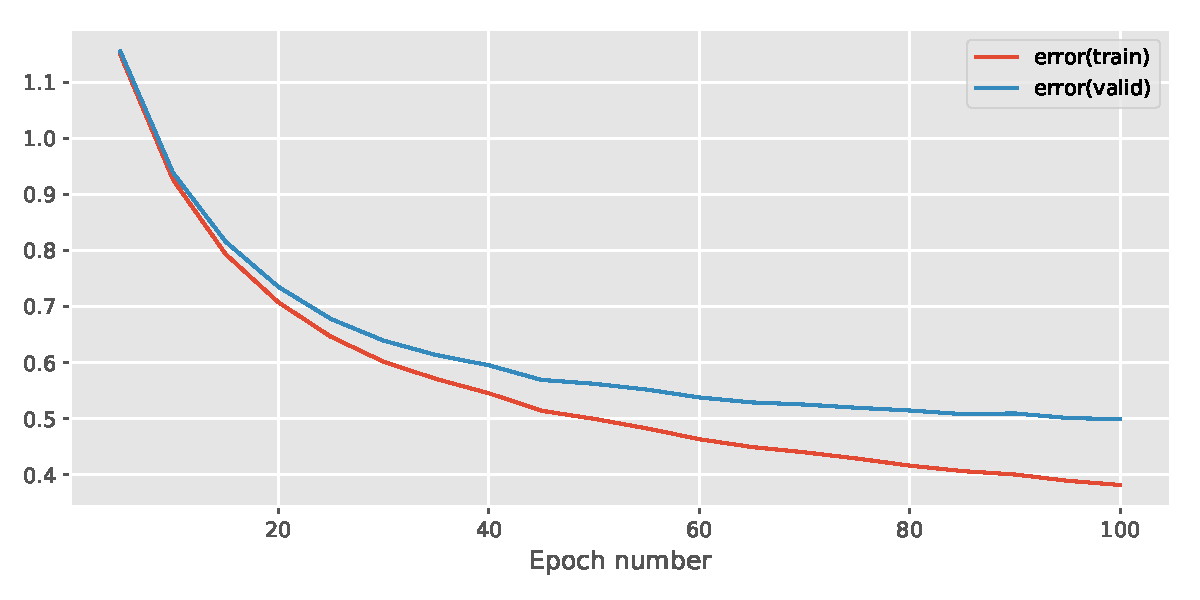
\includegraphics[width=\textwidth]{{../notebooks/figs/gradientdescentlearningrule-num_epochs100-lr0.01-n_hidden2_error}.pdf}
	\end{subfigure}%
	\begin{subfigure}{.17\textwidth}
		\centering
		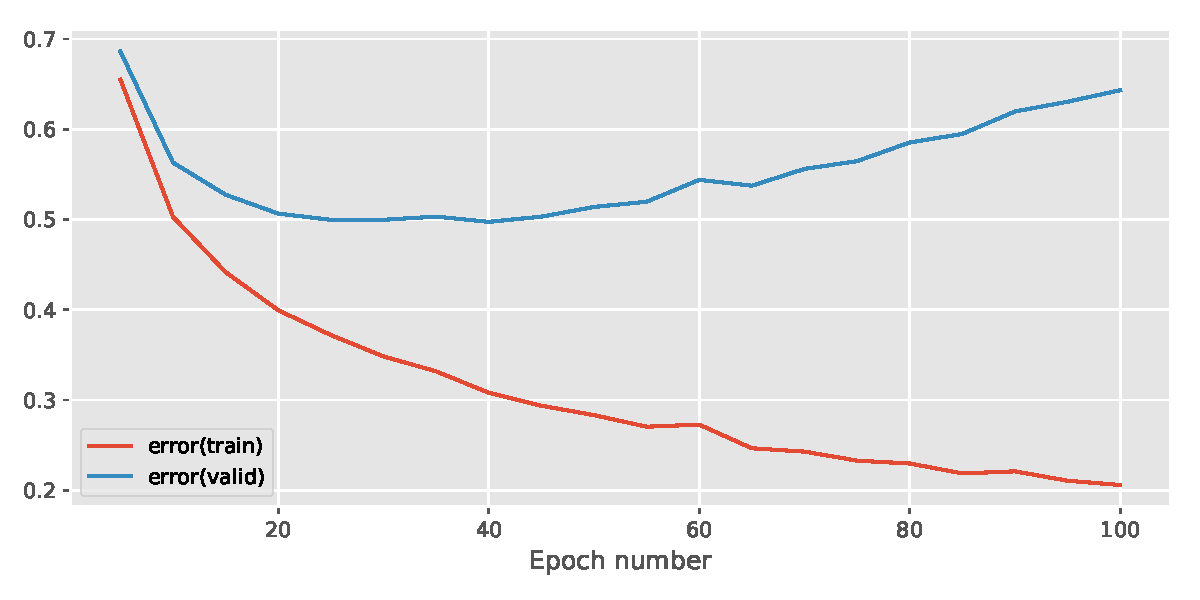
\includegraphics[width=\textwidth]{{../notebooks/figs/gradientdescentlearningrule-num_epochs100-lr0.05-n_hidden2_error}.pdf}
	\end{subfigure}%
	\begin{subfigure}{.17\textwidth}
		\centering
		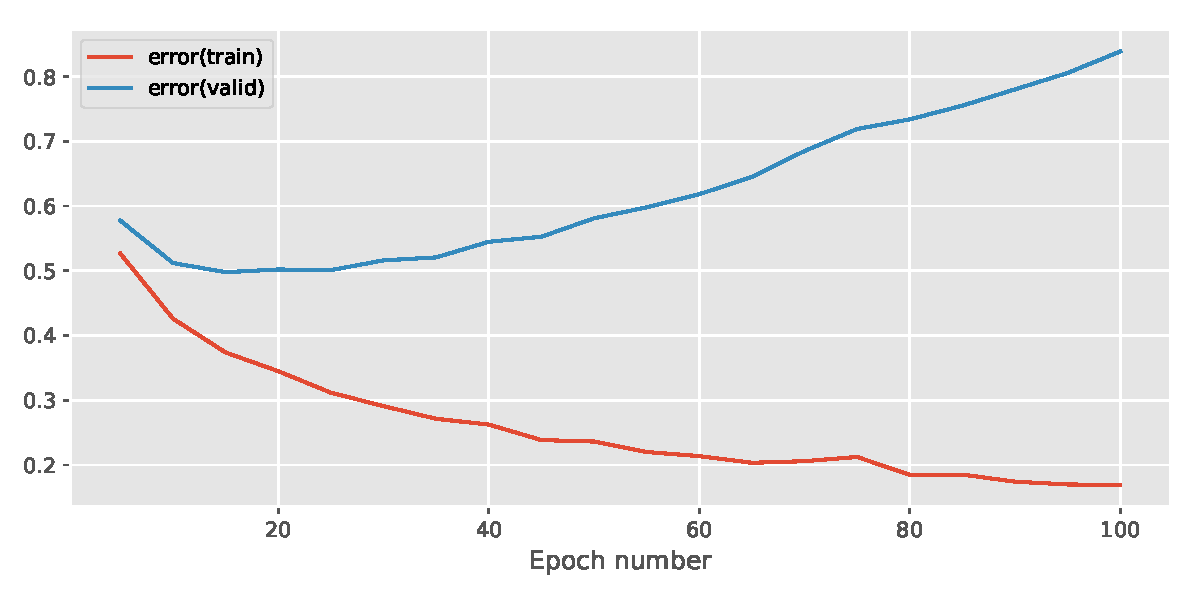
\includegraphics[width=\textwidth]{{../notebooks/figs/gradientdescentlearningrule-num_epochs100-lr0.1-n_hidden2_error}.pdf}
	\end{subfigure}%
	\begin{subfigure}{.17\textwidth}
		\centering
		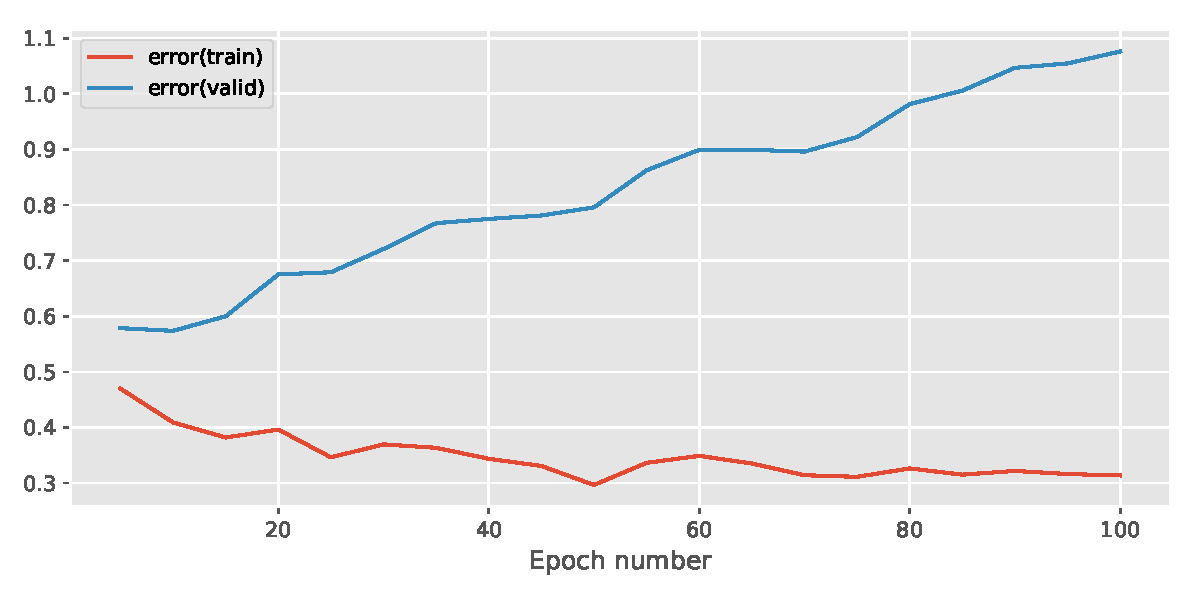
\includegraphics[width=\textwidth]{{../notebooks/figs/gradientdescentlearningrule-num_epochs100-lr0.5-n_hidden2_error}.pdf}
	\end{subfigure}%
	\begin{subfigure}{.17\textwidth}
		\centering
		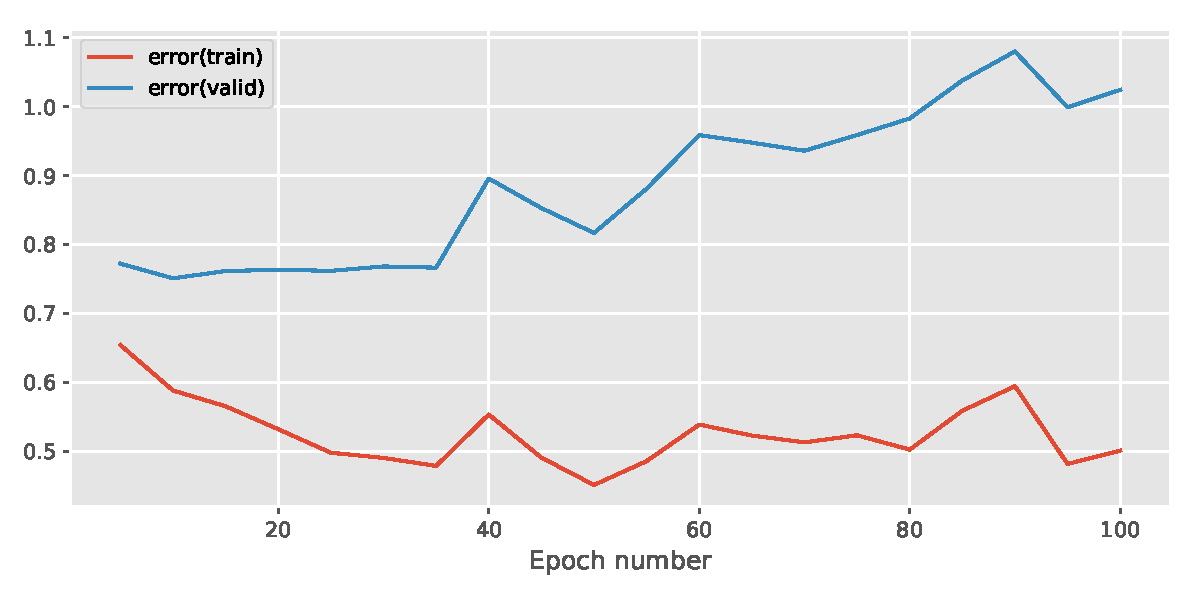
\includegraphics[width=\textwidth]{{../notebooks/figs/gradientdescentlearningrule-num_epochs100-lr1-n_hidden2_error}.pdf}
	\end{subfigure}%
	\caption[short]{Baseline with 2 hidden layers, 100 epochs and $\eta = \lbrace0.01, 0.05, 0.1, 0.5, 1\rbrace$}

	\centering
	\begin{subfigure}{.17\textwidth}
		\centering
		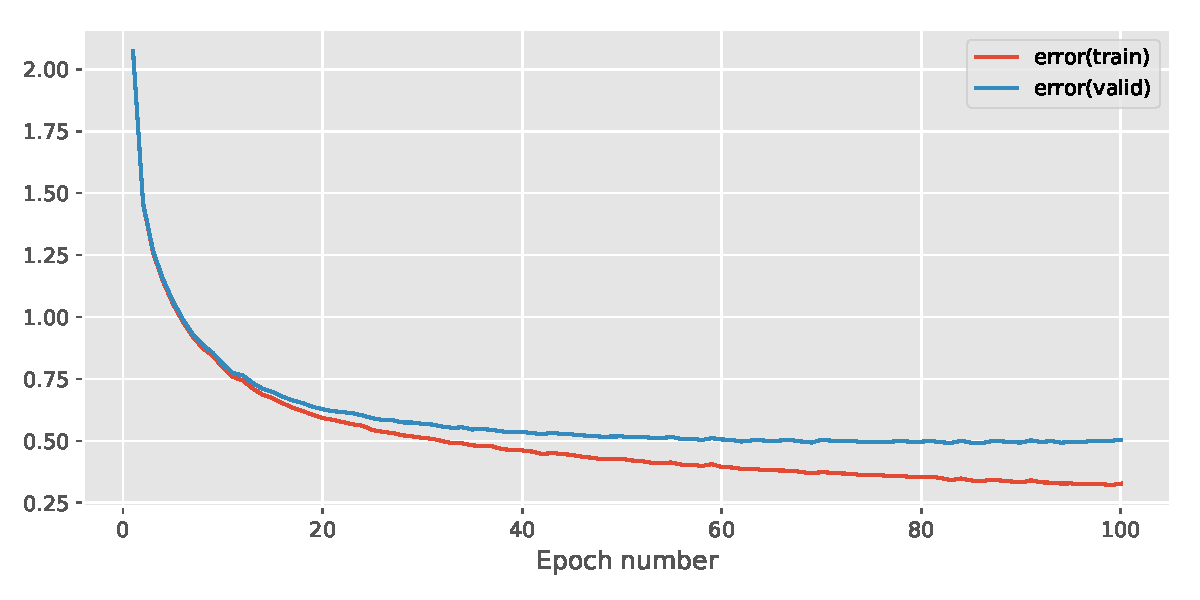
\includegraphics[width=\textwidth]{{../notebooks/figs/gradientdescentlearningrule-num_epochs100-lr0.01-n_hidden3_error}.pdf}
	\end{subfigure}%
	\begin{subfigure}{.17\textwidth}
		\centering
		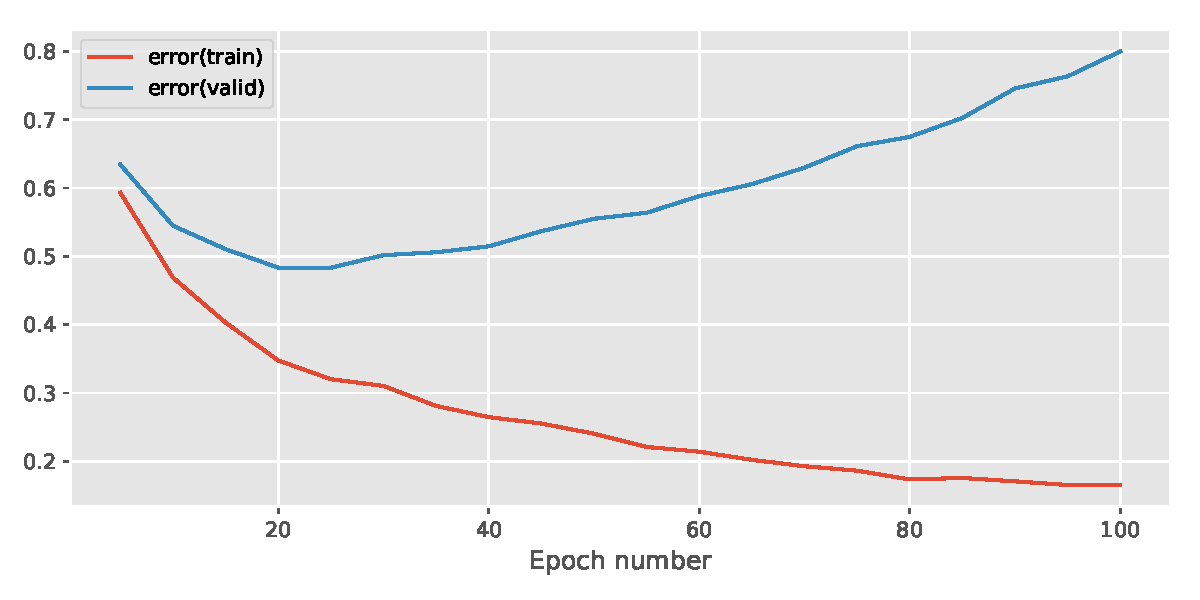
\includegraphics[width=\textwidth]{{../notebooks/figs/gradientdescentlearningrule-num_epochs100-lr0.05-n_hidden3_error}.pdf}
	\end{subfigure}%
	\begin{subfigure}{.17\textwidth}
		\centering
		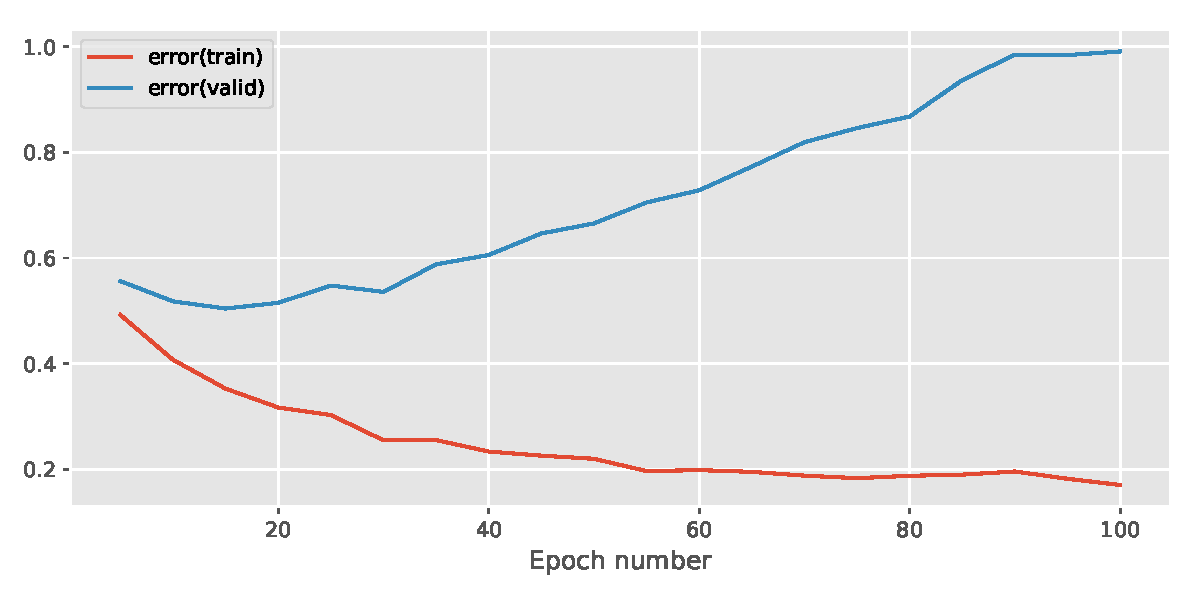
\includegraphics[width=\textwidth]{{../notebooks/figs/gradientdescentlearningrule-num_epochs100-lr0.1-n_hidden3_error}.pdf}
	\end{subfigure}%
	\begin{subfigure}{.17\textwidth}
		\centering
		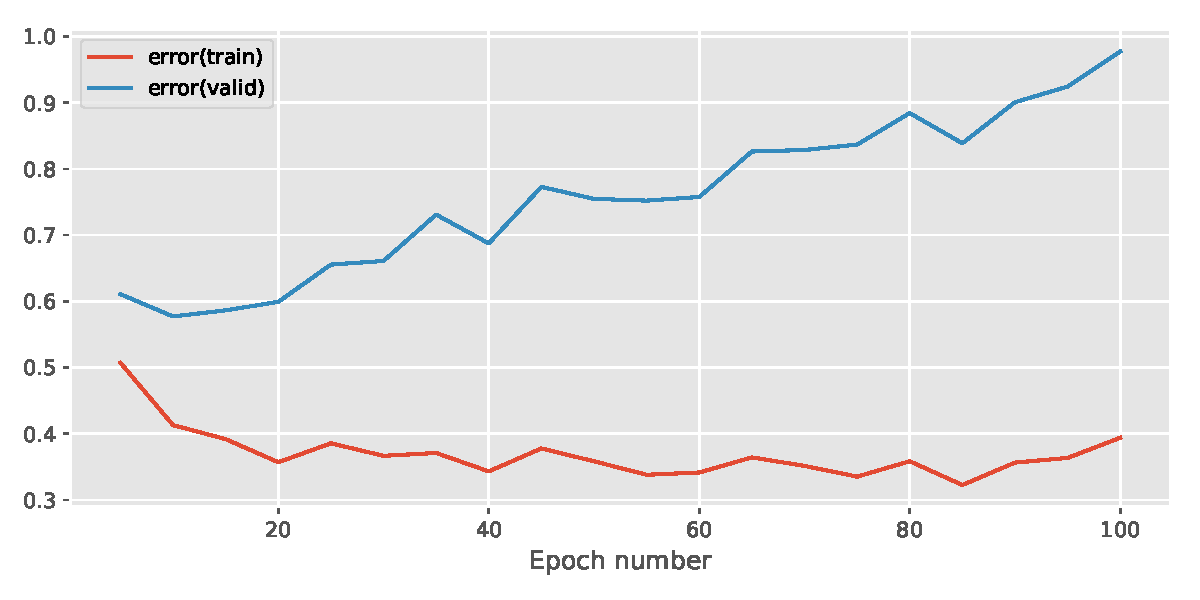
\includegraphics[width=\textwidth]{{../notebooks/figs/gradientdescentlearningrule-num_epochs100-lr0.5-n_hidden3_error}.pdf}
	\end{subfigure}%
	\begin{subfigure}{.17\textwidth}
		\centering
		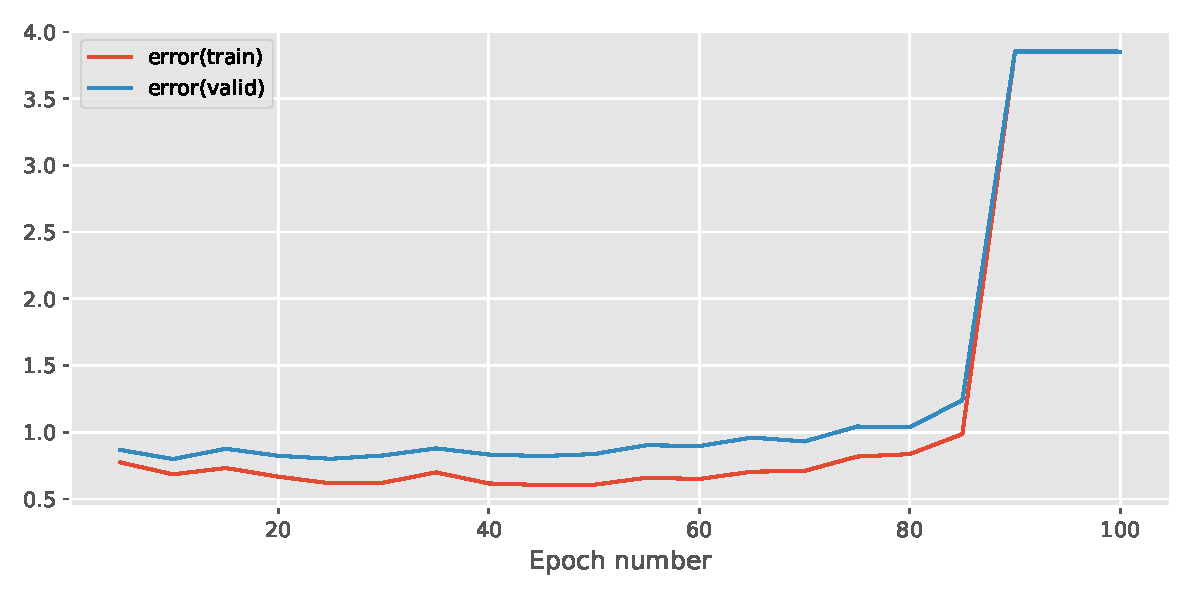
\includegraphics[width=\textwidth]{{../notebooks/figs/gradientdescentlearningrule-num_epochs100-lr1-n_hidden3_error}.pdf}
	\end{subfigure}%
	\caption[short]{Baseline with 3 hidden layers, 100 epochs and $\eta = \lbrace0.01, 0.05, 0.1, 0.5, 1\rbrace$}

	\centering
	\begin{subfigure}{.17\textwidth}
		\centering
		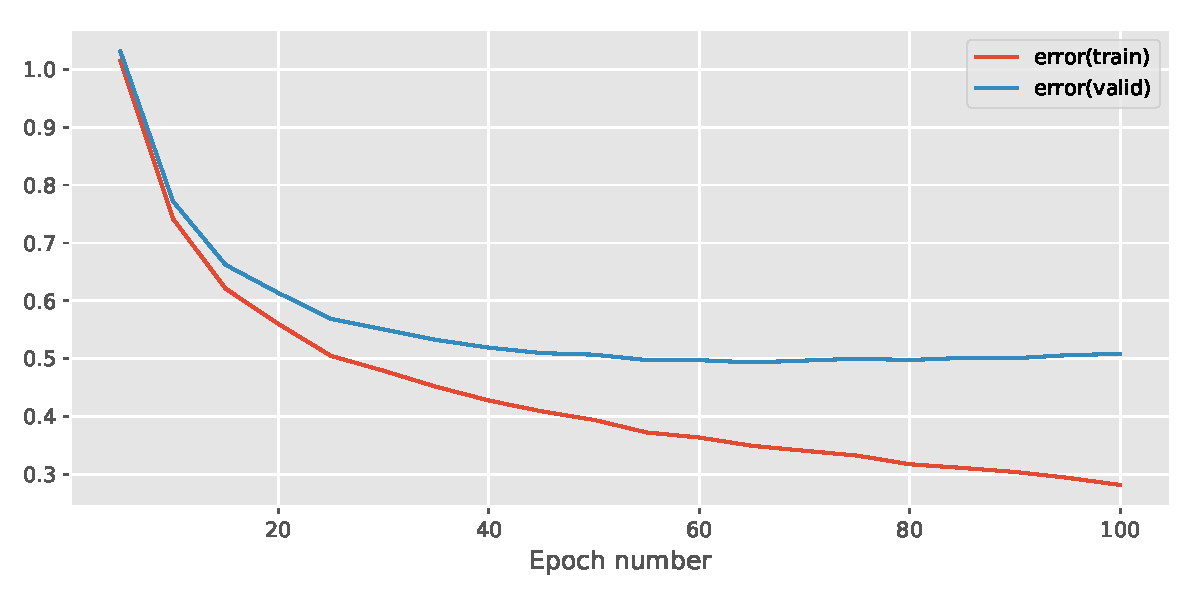
\includegraphics[width=\textwidth]{{../notebooks/figs/gradientdescentlearningrule-num_epochs100-lr0.01-n_hidden4_error}.pdf}
	\end{subfigure}%
	\begin{subfigure}{.17\textwidth}
		\centering
		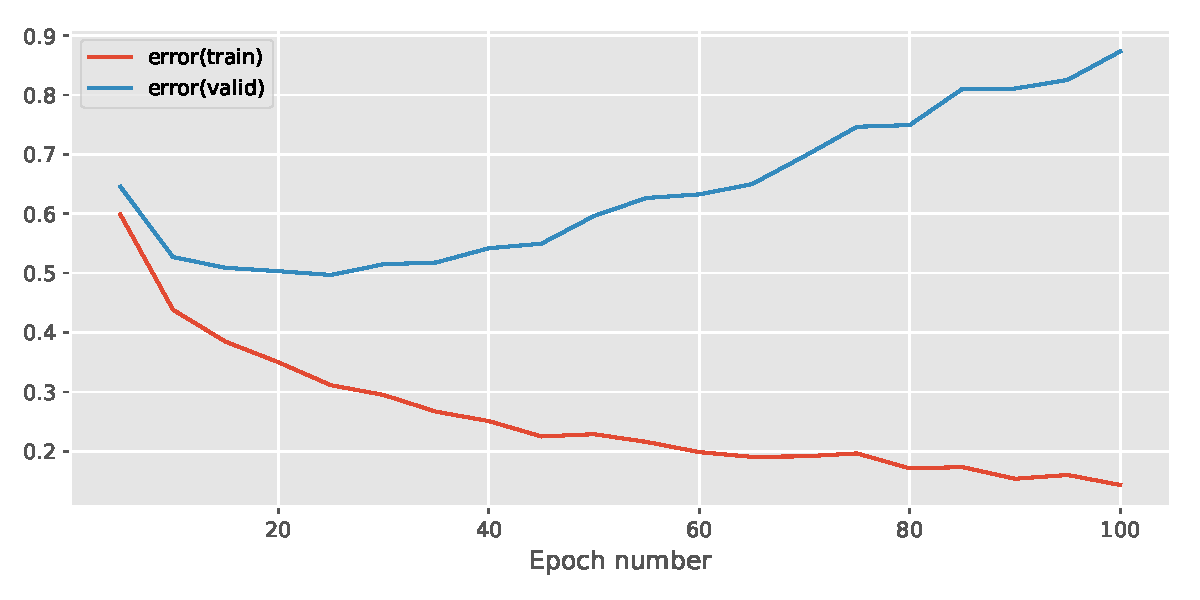
\includegraphics[width=\textwidth]{{../notebooks/figs/gradientdescentlearningrule-num_epochs100-lr0.05-n_hidden4_error}.pdf}
	\end{subfigure}%
	\begin{subfigure}{.17\textwidth}
		\centering
		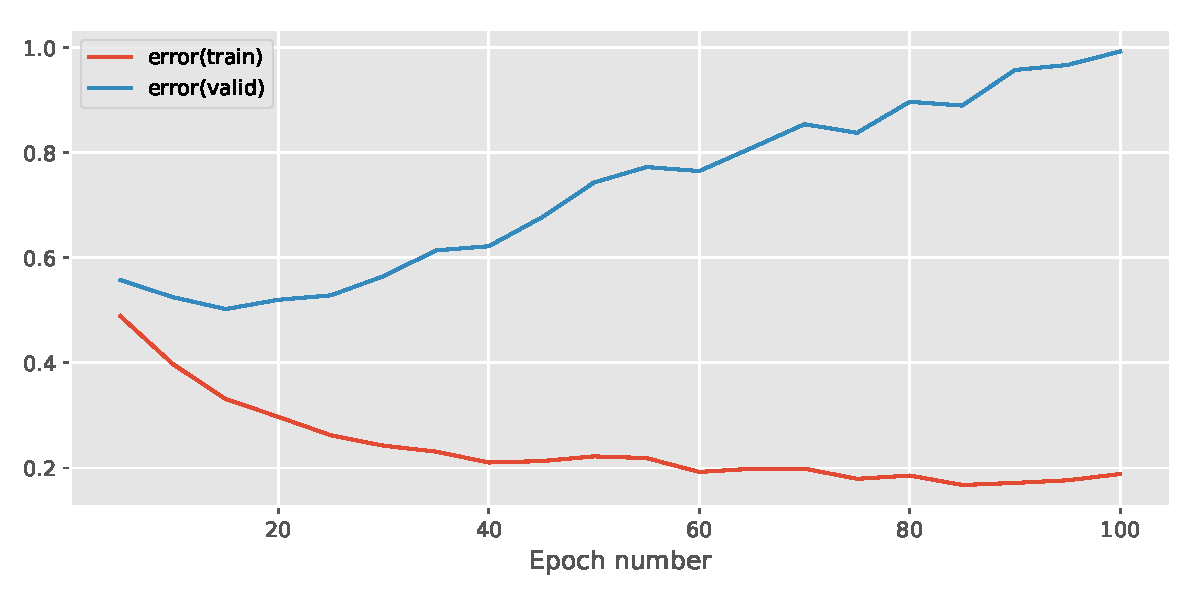
\includegraphics[width=\textwidth]{{../notebooks/figs/gradientdescentlearningrule-num_epochs100-lr0.1-n_hidden4_error}.pdf}
	\end{subfigure}%
	\begin{subfigure}{.17\textwidth}
		\centering
		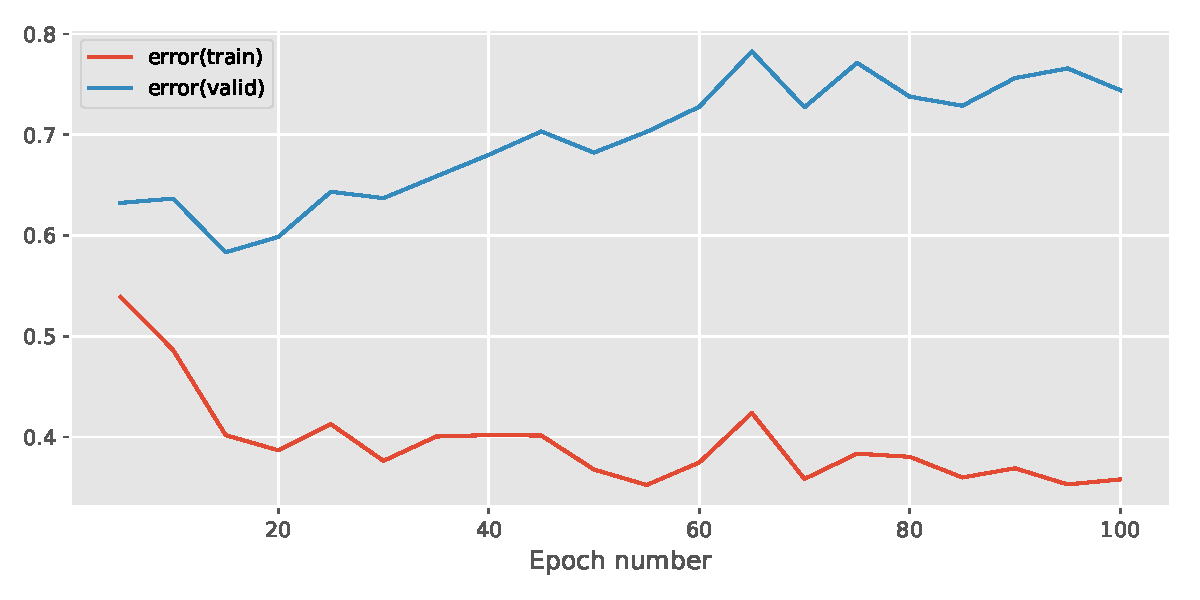
\includegraphics[width=\textwidth]{{../notebooks/figs/gradientdescentlearningrule-num_epochs100-lr0.5-n_hidden4_error}.pdf}
	\end{subfigure}%
	\begin{subfigure}{.17\textwidth}
		\centering
		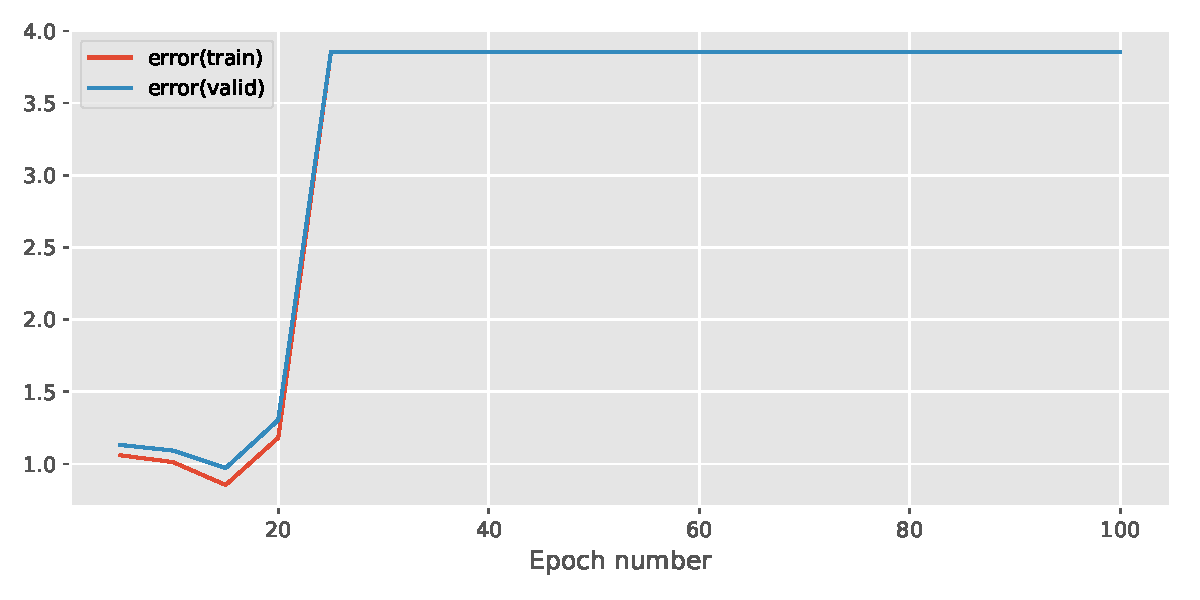
\includegraphics[width=\textwidth]{{../notebooks/figs/gradientdescentlearningrule-num_epochs100-lr1-n_hidden4_error}.pdf}
	\end{subfigure}%
	\caption[short]{Baseline with 4 hidden layers, 100 epochs and $\eta = \lbrace0.01, 0.05, 0.1, 0.5, 1\rbrace$}

	\centering
	\begin{subfigure}{.17\textwidth}
		\centering
		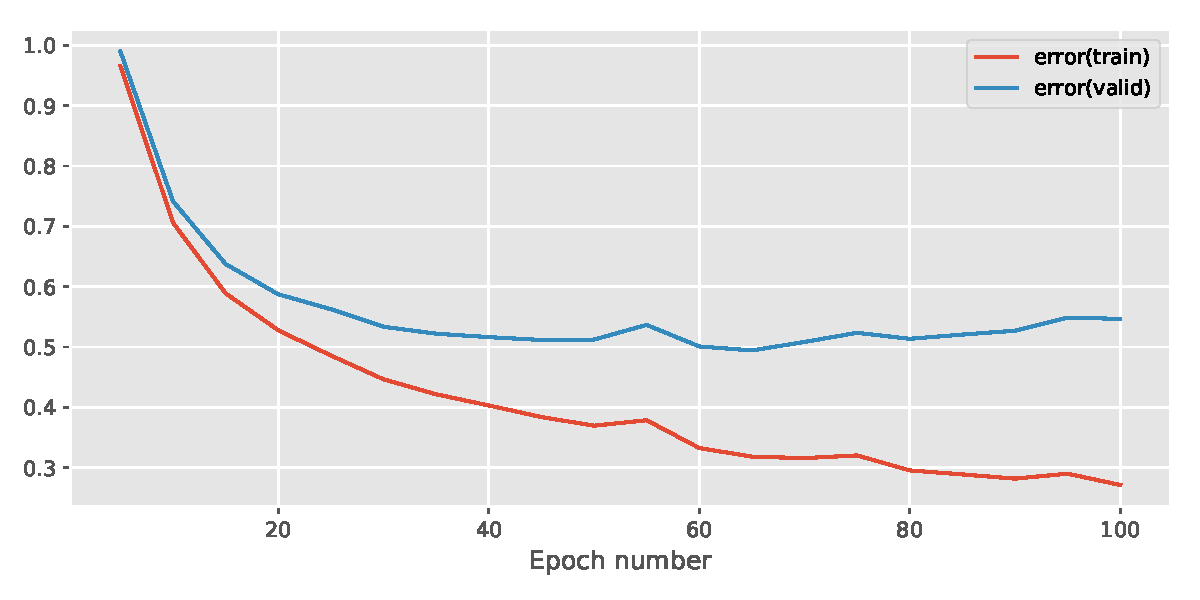
\includegraphics[width=\textwidth]{{../notebooks/figs/gradientdescentlearningrule-num_epochs100-lr0.01-n_hidden5_error}.pdf}
	\end{subfigure}%
	\begin{subfigure}{.17\textwidth}
		\centering
		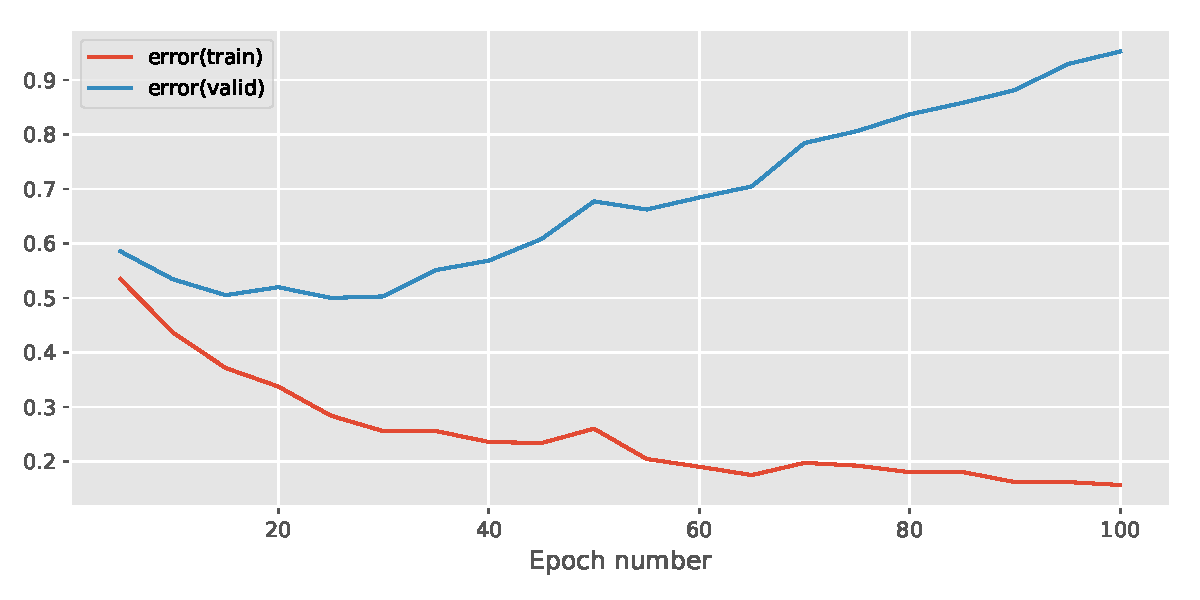
\includegraphics[width=\textwidth]{{../notebooks/figs/gradientdescentlearningrule-num_epochs100-lr0.05-n_hidden5_error}.pdf}
	\end{subfigure}%
	\begin{subfigure}{.17\textwidth}
		\centering
		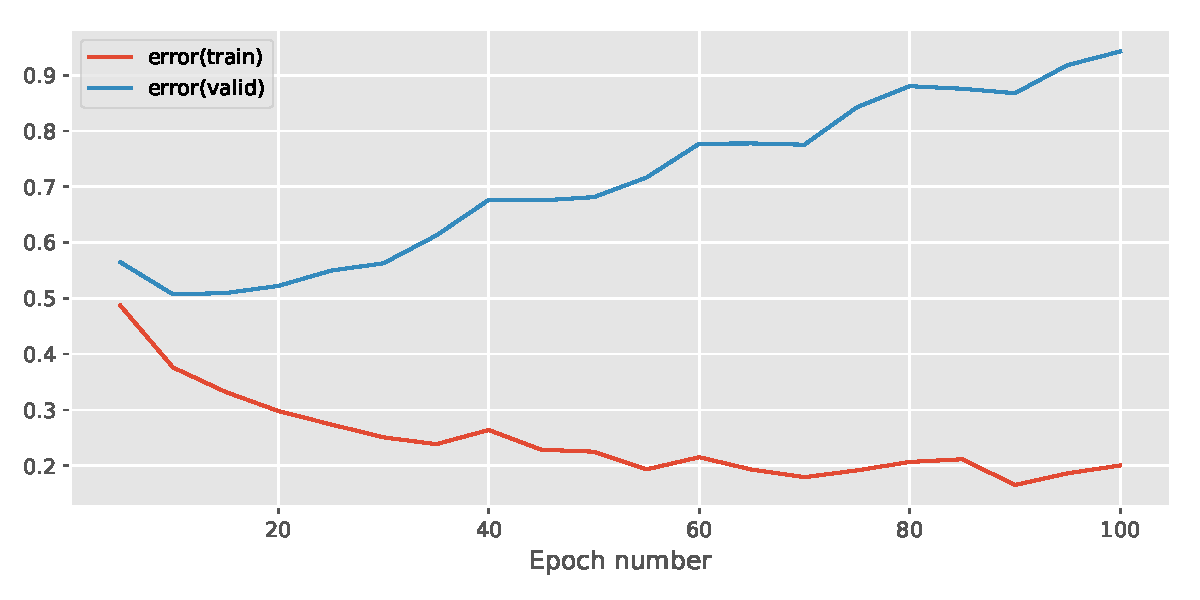
\includegraphics[width=\textwidth]{{../notebooks/figs/gradientdescentlearningrule-num_epochs100-lr0.1-n_hidden5_error}.pdf}
	\end{subfigure}%
	\begin{subfigure}{.17\textwidth}
		\centering
		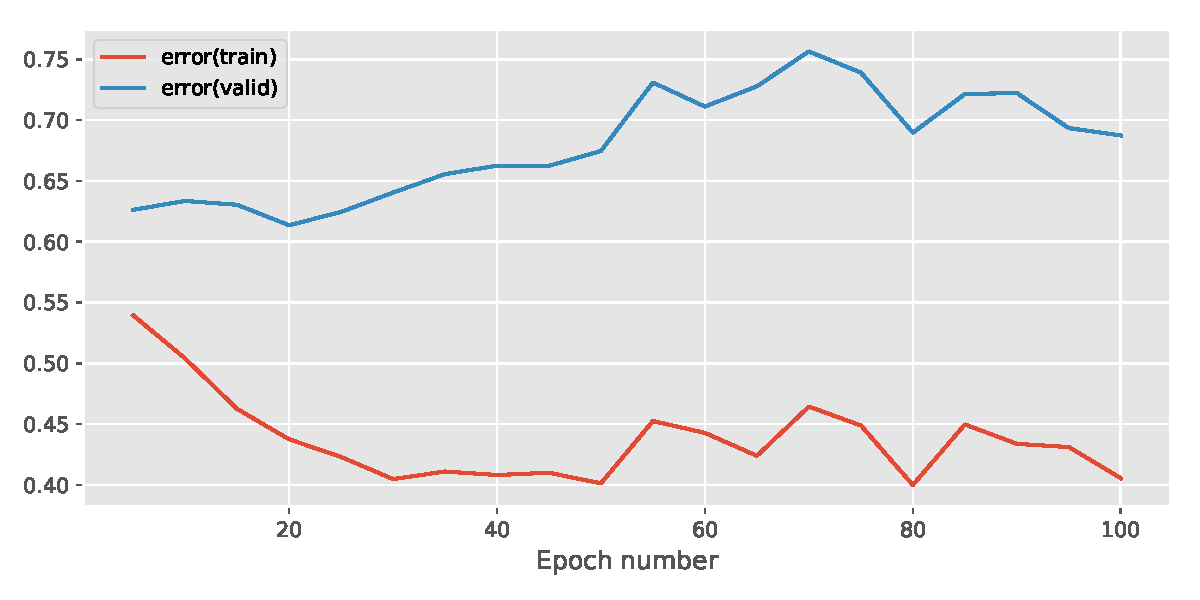
\includegraphics[width=\textwidth]{{../notebooks/figs/gradientdescentlearningrule-num_epochs100-lr0.5-n_hidden5_error}.pdf}
	\end{subfigure}%
	\begin{subfigure}{.17\textwidth}
		\centering
		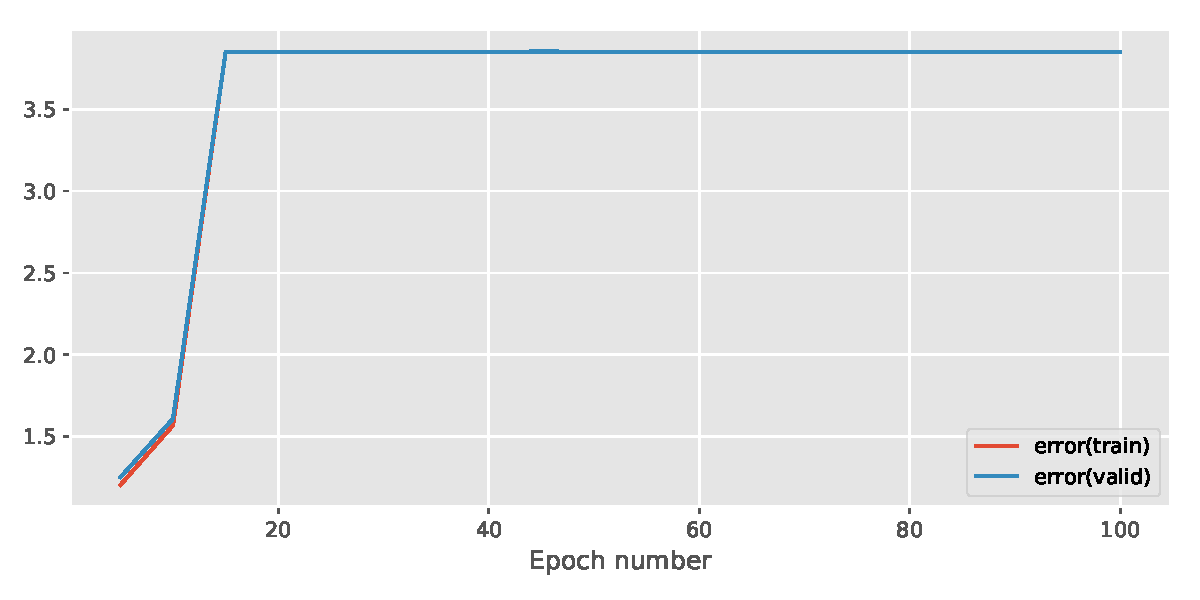
\includegraphics[width=\textwidth]{{../notebooks/figs/gradientdescentlearningrule-num_epochs100-lr1-n_hidden5_error}.pdf}
	\end{subfigure}%
	\caption[short]{Baseline with 5 hidden layers, 100 epochs and $\eta = \lbrace0.01, 0.05, 0.1, 0.5, 1\rbrace$}
\end{sidewaysfigure*}


\begin{sidewaysfigure*}
	\centering
	\begin{subfigure}{.2\textwidth}
		\centering
		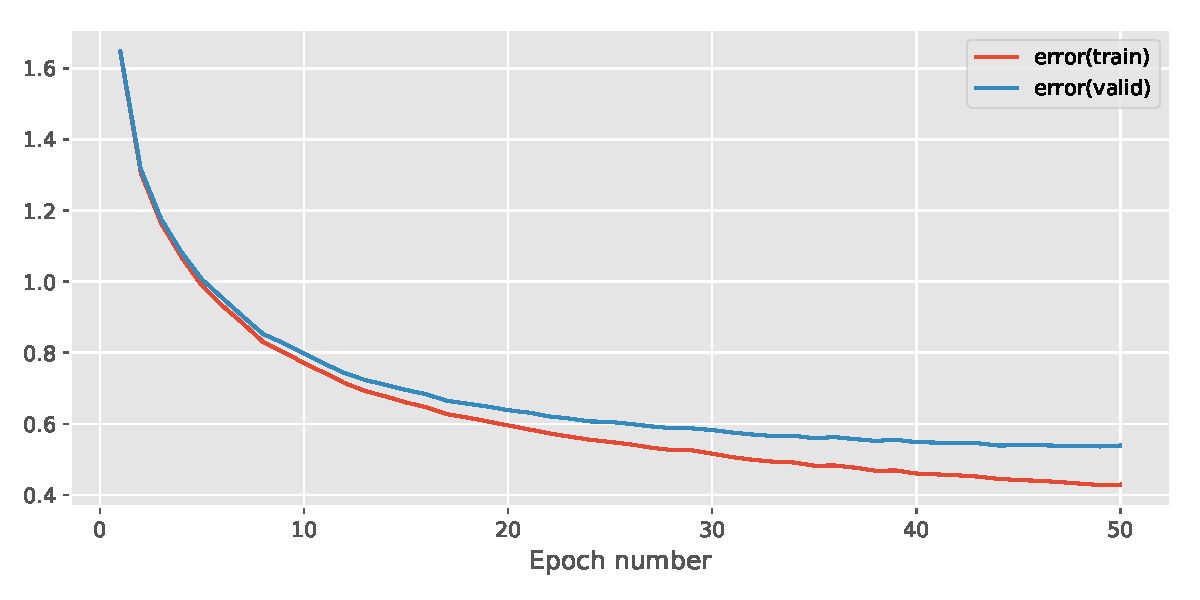
\includegraphics[width=\textwidth]{{../notebooks/figs/rmsproplearningrule-num_epochs50-lr0.0001-n_hidden3_error}.pdf}
	\end{subfigure}%
	\begin{subfigure}{.2\textwidth}
		\centering
		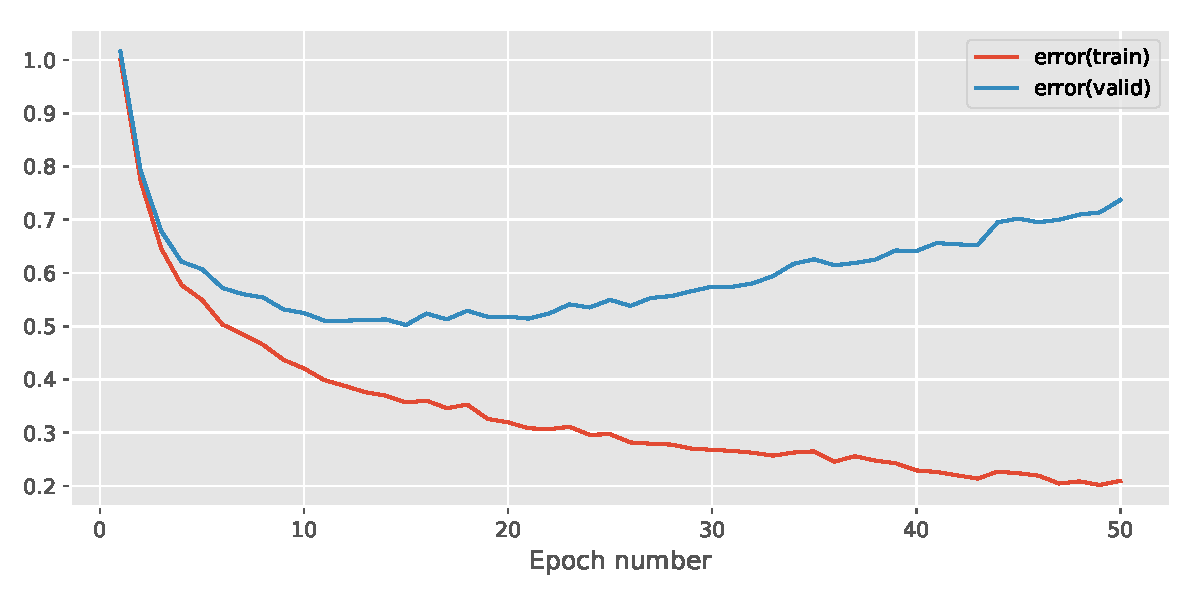
\includegraphics[width=\textwidth]{{../notebooks/figs/rmsproplearningrule-num_epochs50-lr0.0005-n_hidden3_error}.pdf}
	\end{subfigure}%
	\begin{subfigure}{.2\textwidth}
		\centering
		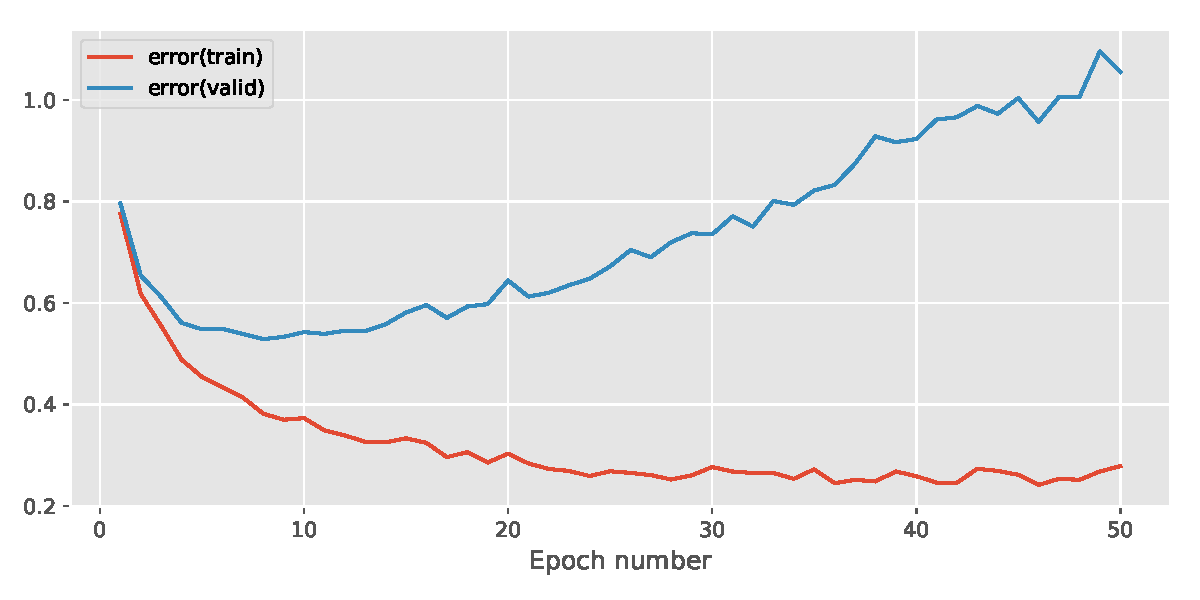
\includegraphics[width=\textwidth]{{../notebooks/figs/rmsproplearningrule-num_epochs50-lr0.001-n_hidden3_error}.pdf}
	\end{subfigure}%
	\begin{subfigure}{.2\textwidth}
		\centering
		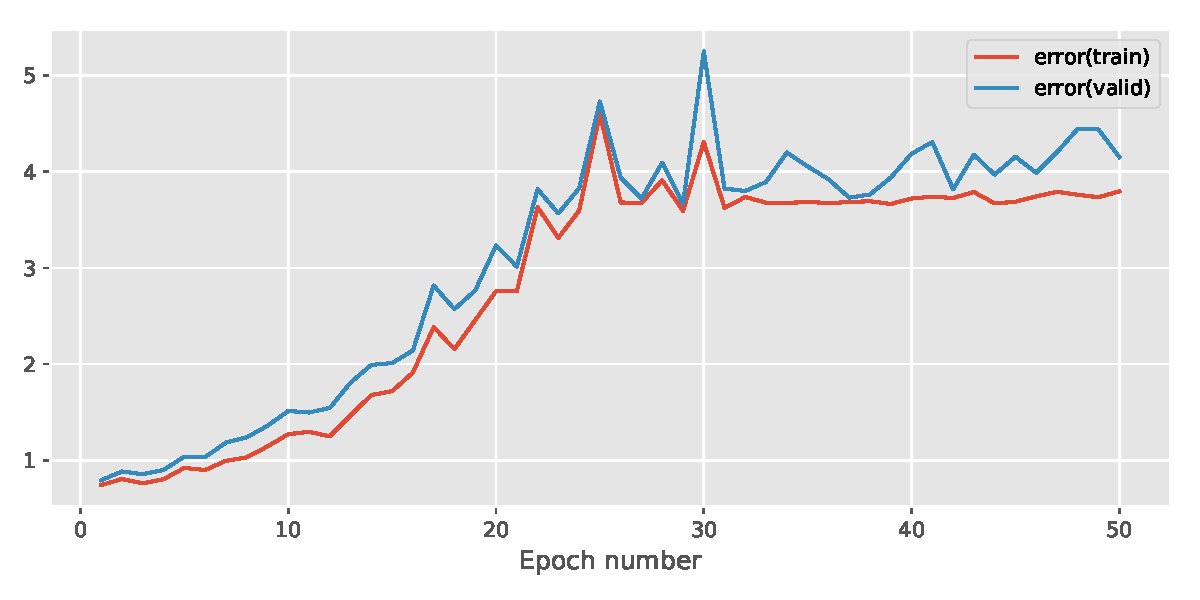
\includegraphics[width=\textwidth]{{../notebooks/figs/rmsproplearningrule-num_epochs50-lr0.005-n_hidden3_error}.pdf}
	\end{subfigure}%
	\begin{subfigure}{.2\textwidth}
		\centering
		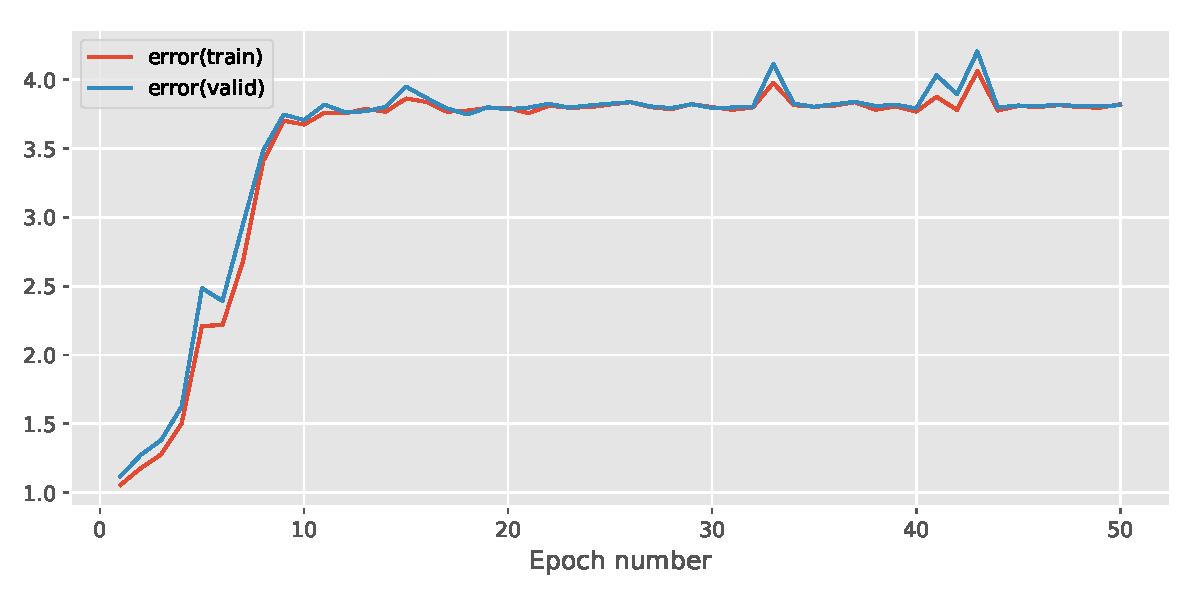
\includegraphics[width=\textwidth]{{../notebooks/figs/rmsproplearningrule-num_epochs50-lr0.01-n_hidden3_error}.pdf}
	\end{subfigure}%
	\caption[short]{RMSprop with 3 hidden layers, 50 epochs and $\eta = \lbrace1\mathrm{e}{-4}, 5\mathrm{e}{-4}, 1\mathrm{e}{-3}, 5\mathrm{e}{-3}, 1\mathrm{e}{-2}\rbrace$}
	\label{fig:rmsprop}

\centering
	\begin{subfigure}{.2\textwidth}
		\centering
		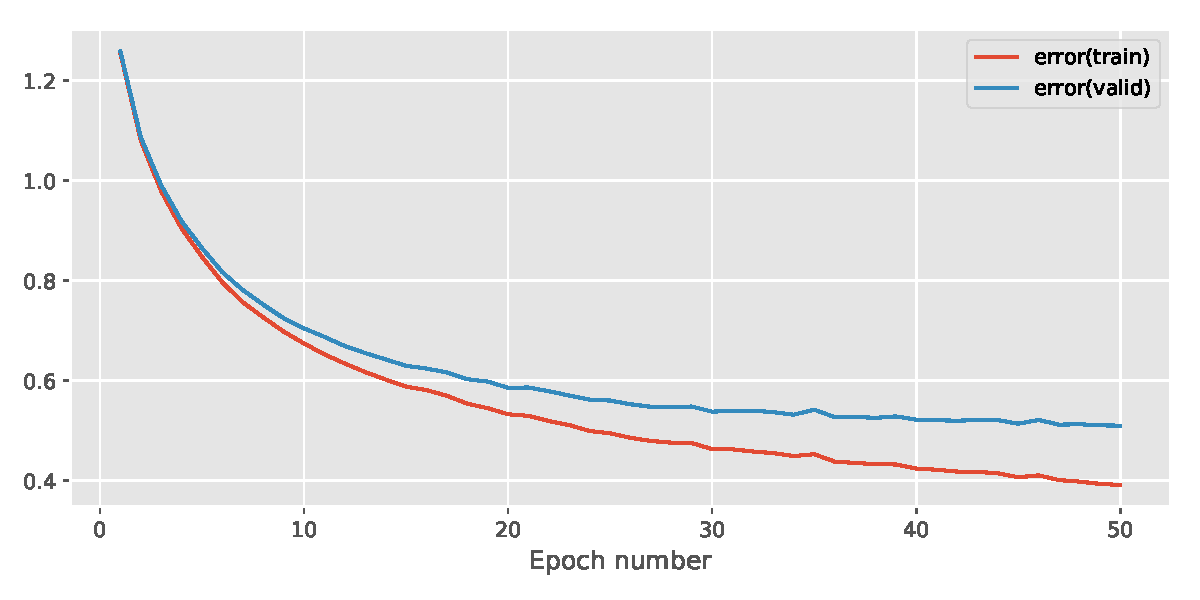
\includegraphics[width=\textwidth]{{../notebooks/figs/adamlearningrule-num_epochs50-lr0.0001-n_hidden3_error}.pdf}
	\end{subfigure}%
	\begin{subfigure}{.2\textwidth}
		\centering
		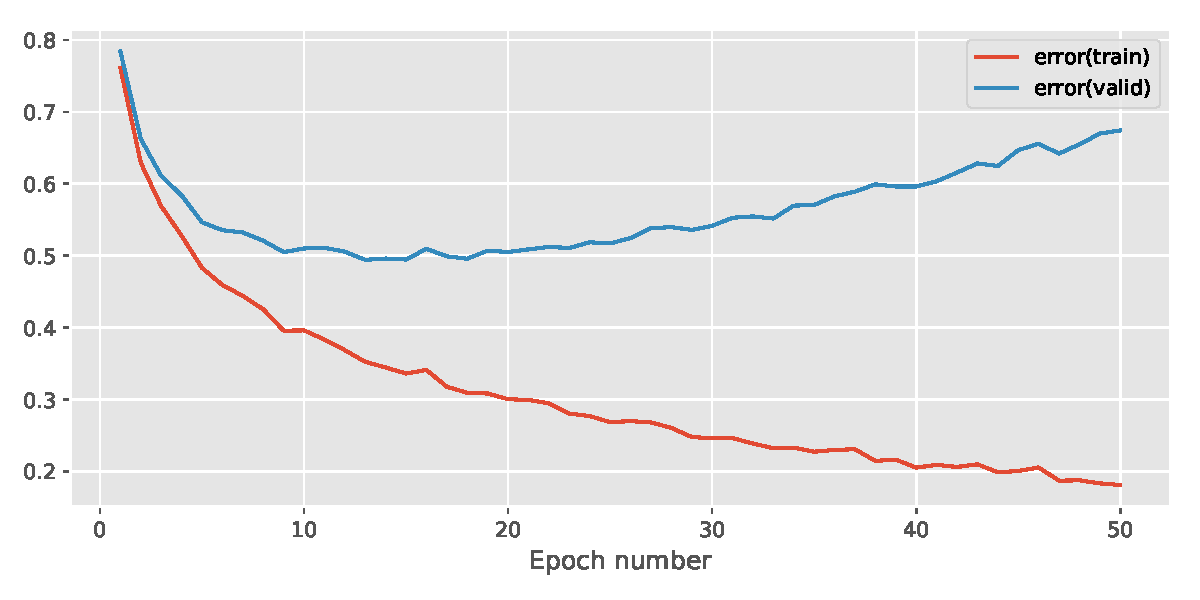
\includegraphics[width=\textwidth]{{../notebooks/figs/adamlearningrule-num_epochs50-lr0.0005-n_hidden3_error}.pdf}
	\end{subfigure}%
	\begin{subfigure}{.2\textwidth}
		\centering
		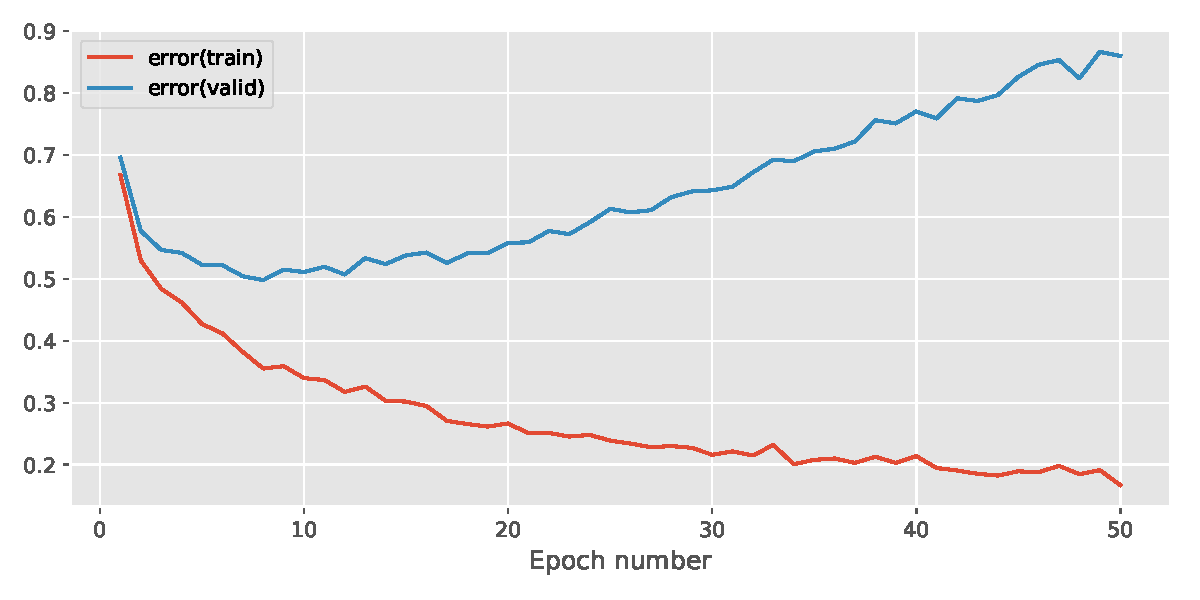
\includegraphics[width=\textwidth]{{../notebooks/figs/adamlearningrule-num_epochs50-lr0.001-n_hidden3_error}.pdf}
	\end{subfigure}%
	\begin{subfigure}{.2\textwidth}
		\centering
		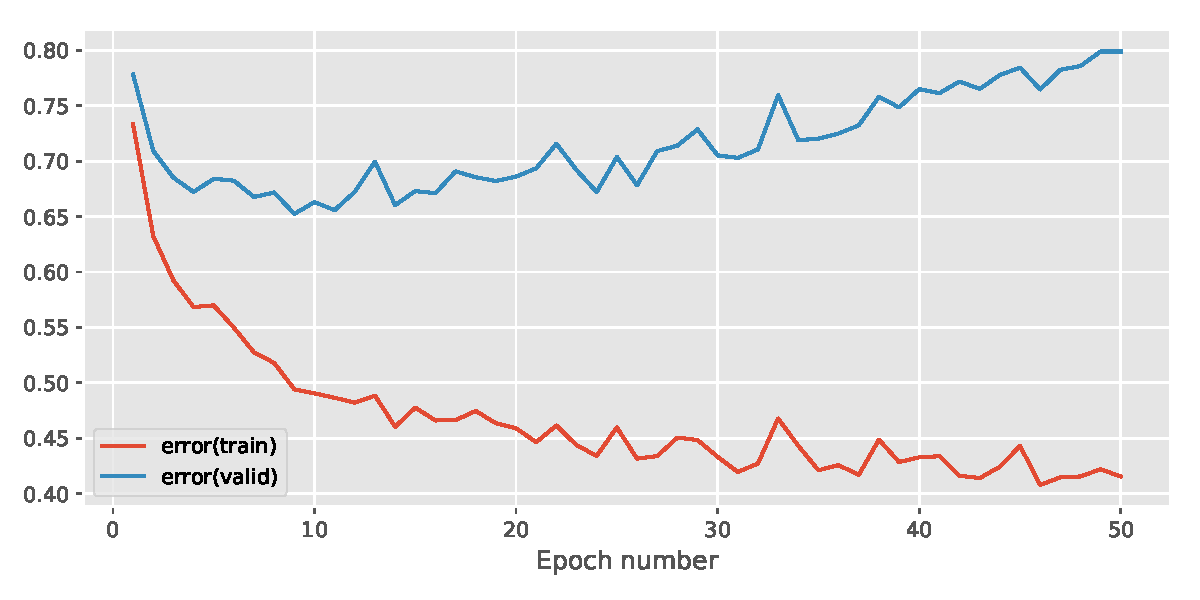
\includegraphics[width=\textwidth]{{../notebooks/figs/adamlearningrule-num_epochs50-lr0.005-n_hidden3_error}.pdf}
	\end{subfigure}%
	\begin{subfigure}{.2\textwidth}
		\centering
		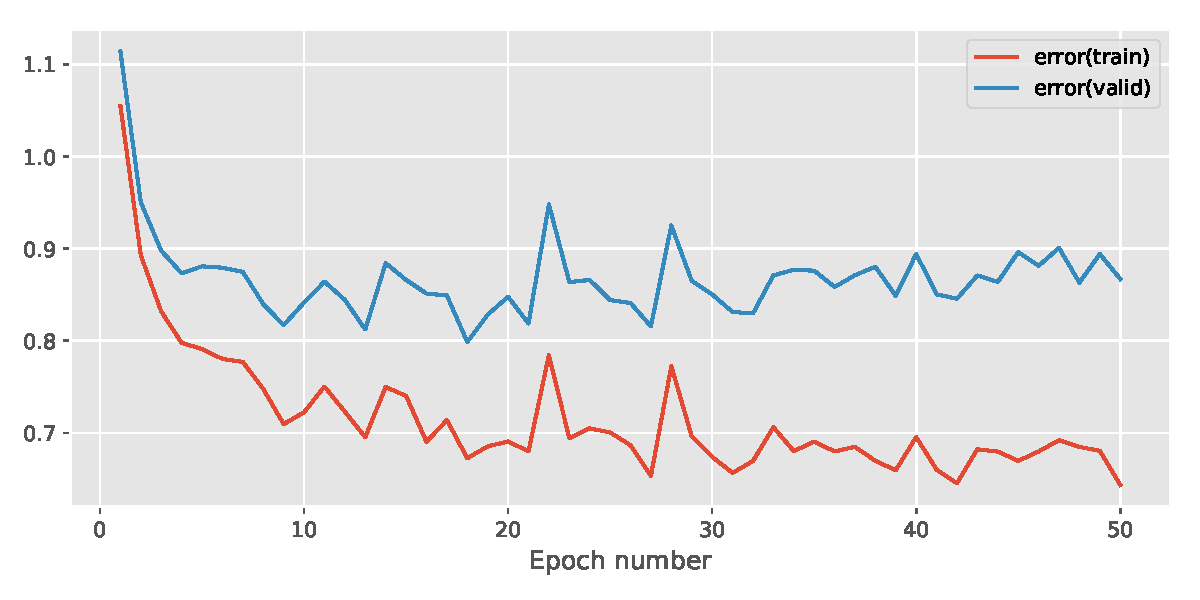
\includegraphics[width=\textwidth]{{../notebooks/figs/adamlearningrule-num_epochs50-lr0.01-n_hidden3_error}.pdf}
	\end{subfigure}%
	\caption[short]{Adam with 3 hidden layers, 50 epochs and $\eta = \lbrace1\mathrm{e}{-4}, 5\mathrm{e}{-4}, 1\mathrm{e}{-3}, 5\mathrm{e}{-3}, 1\mathrm{e}{-2}\rbrace$}
	\label{fig:adam}
\end{sidewaysfigure*}

\begin{figure*}
	\centering
	\begin{subfigure}{.45\textwidth}
		\centering
		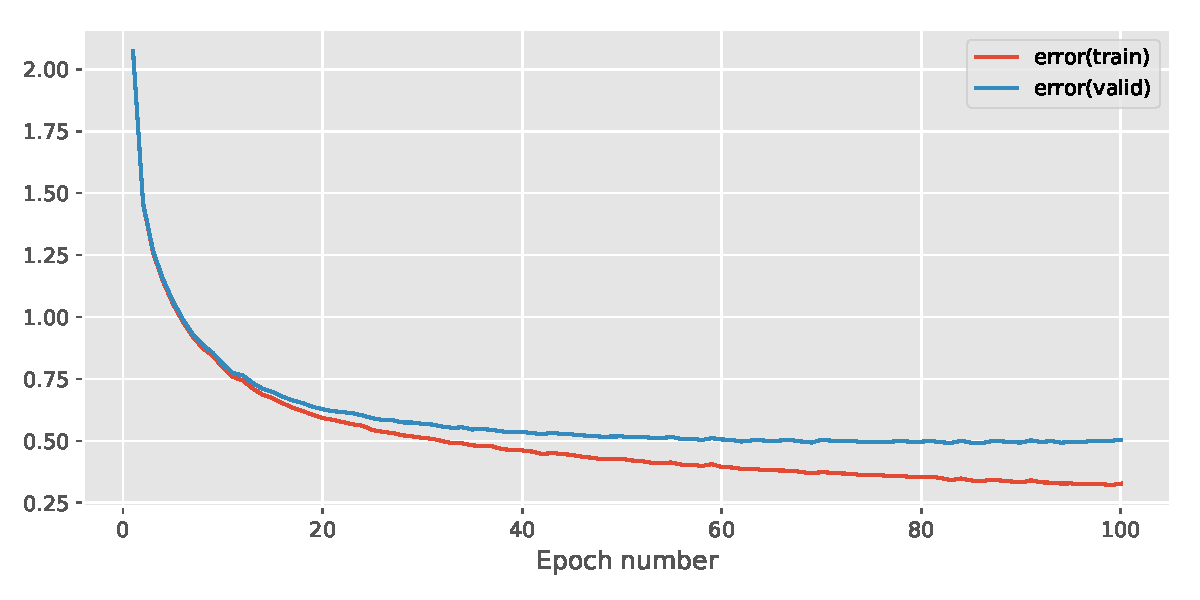
\includegraphics[width=\textwidth]{{../notebooks/figs/gradientdescentlearningrule-num_epochs100-lr0.01-n_hidden3_error}.pdf}
		\caption[short]{SGD baseline, $lr_{max=0.01}$}
	\end{subfigure}%
	\begin{subfigure}{.45\textwidth}
		\centering
		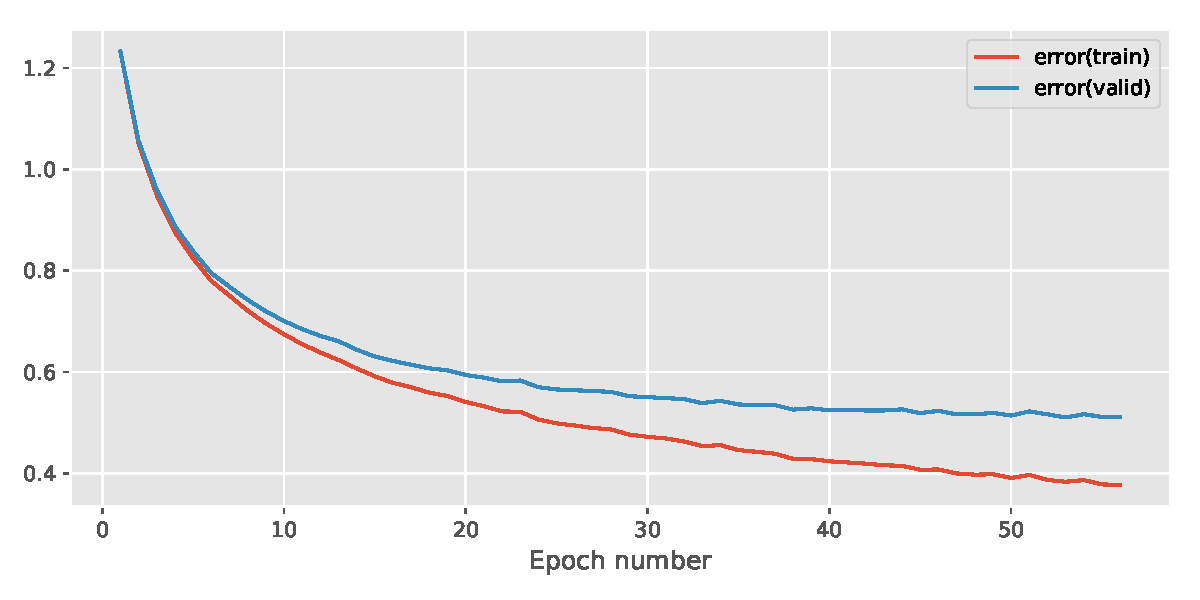
\includegraphics[width=\textwidth]{{../notebooks/figs/adamlearningrule-num_epochs99-lr0.0001-n_hidden3_error}.pdf}
		\caption[short]{Adam baseline, $lr_{max=0.0001}$}
	\end{subfigure}%

	\begin{subfigure}{.45\textwidth}
		\centering
		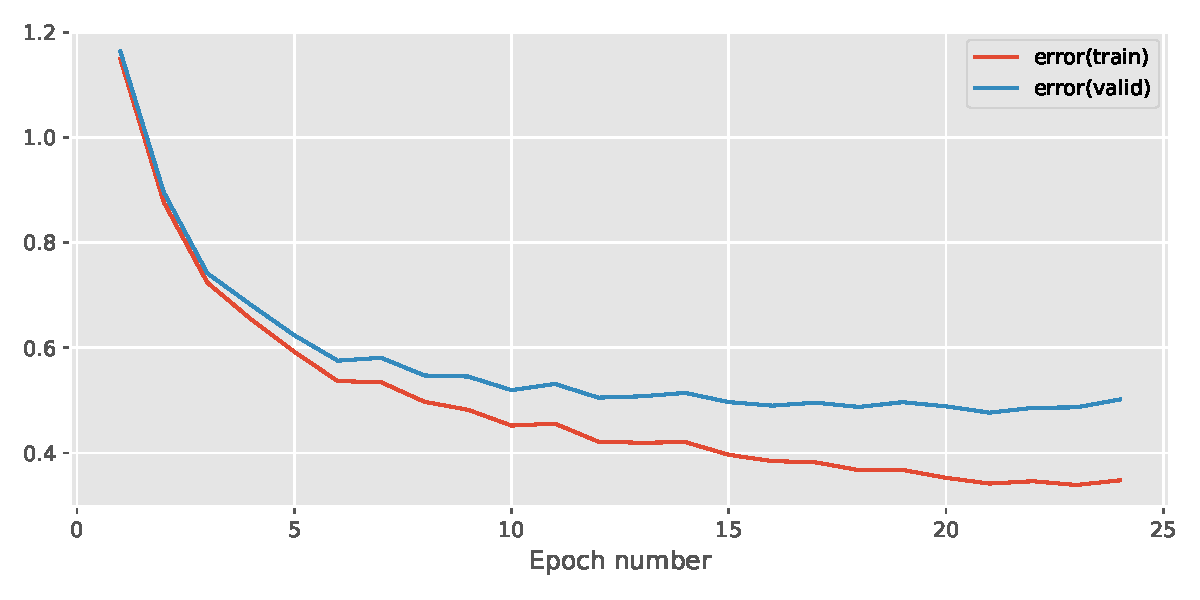
\includegraphics[width=\textwidth]{{../notebooks/figs/gradientdescentlearningrule-norestart-num_epochs100-lr0.05-n_hidden3_error}.pdf}
		\caption[short]{SGD annealed with no restart, $lr_{max=0.01}$}
	\end{subfigure}%
	\begin{subfigure}{.45\textwidth}
		\centering
		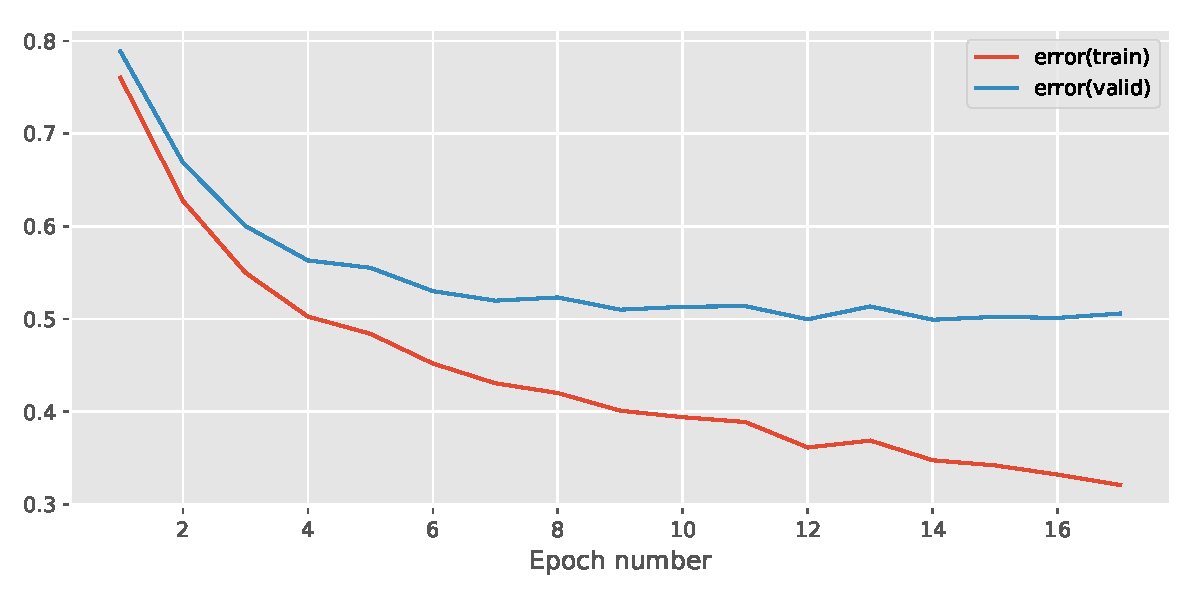
\includegraphics[width=\textwidth]{{../notebooks/figs/adamlearningrule-norestart-num_epochs100-lr0.0005-n_hidden3_error}.pdf}
		\caption[short]{Adam annealed with no restart, $lr_{max=0.0001}$}
	\end{subfigure}%
	\label{fig:norestart}
	
	\begin{subfigure}{.45\textwidth}
		\centering
		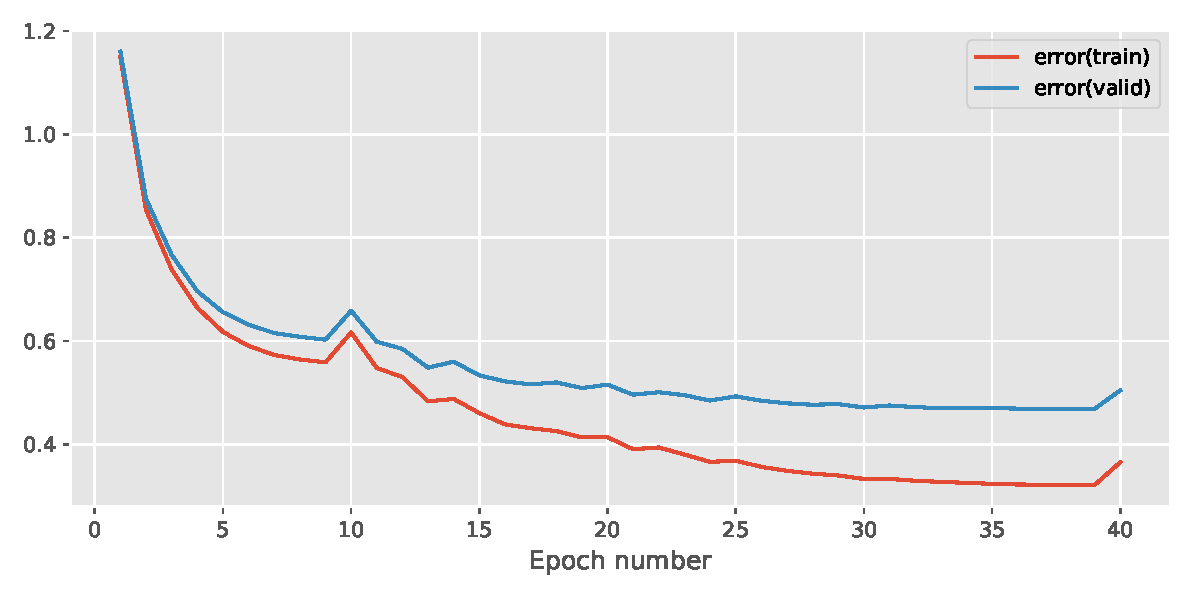
\includegraphics[width=\textwidth]{{../notebooks/figs/gradientdescentlearningrule-restart-num_epochs100-lr0.05-n_hidden3_error}.pdf}
		\caption[short]{SGD annealed with warm restart, $lr_{max=0.01}$}
	\end{subfigure}%
	\begin{subfigure}{.45\textwidth}
		\centering
		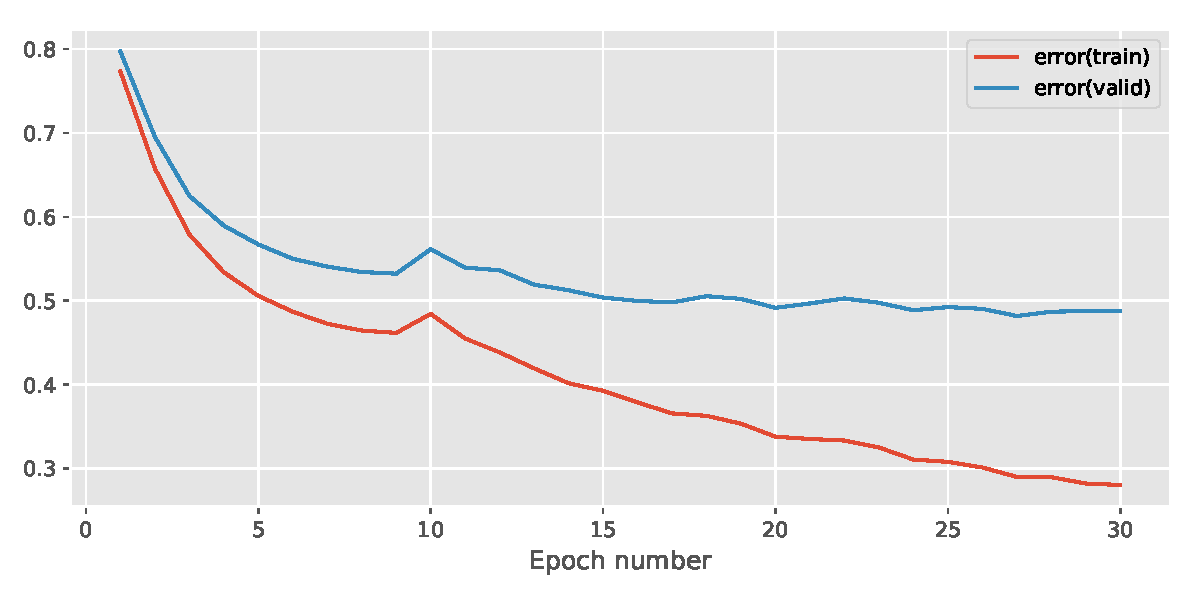
\includegraphics[width=\textwidth]{{../notebooks/figs/adamlearningrule-restart-num_epochs100-lr0.0005-n_hidden3_error}.pdf}
		\caption[short]{Adam annealed with warm restart, $lr_{max=0.0001}$}
	\end{subfigure}%
	\caption[short]{A comparison of no learning rate annealing, annealing with no restart and annealing with restarts. SGD \& Adam optimizer on 3 hidden layer ReLU networks.}
	\label{fig:restart}
\end{figure*}

\begin{figure*}
	\centering
	\begin{subfigure}{.45\textwidth}
		\centering
		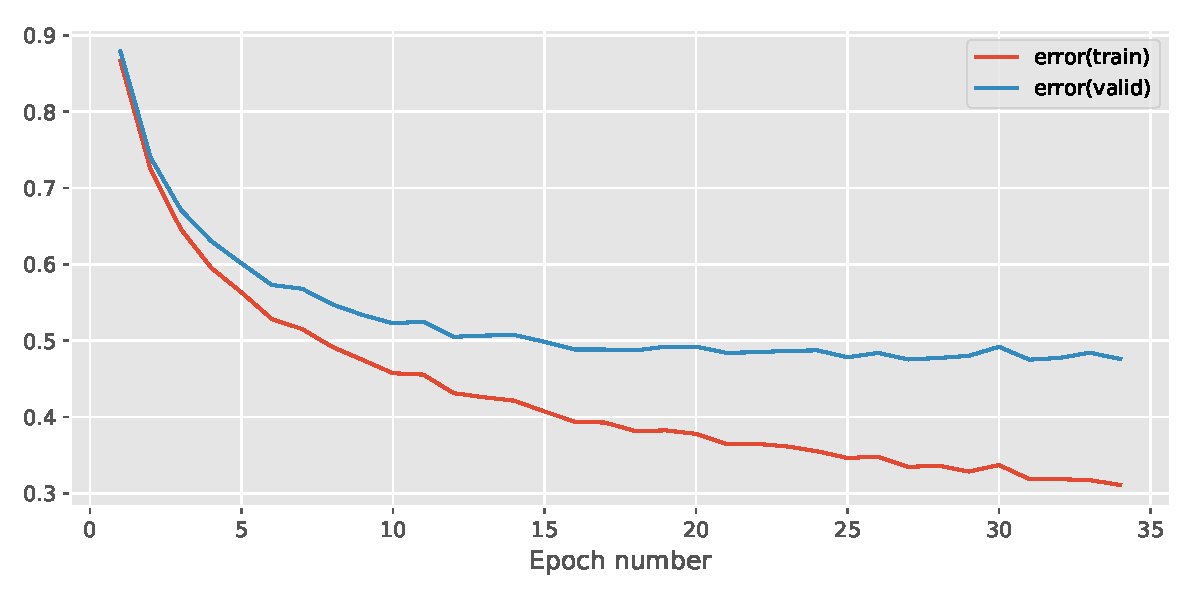
\includegraphics[width=\textwidth]{{../notebooks/figs/adamlearningrulewithweightdecay-constantlearningratescheduler-nonetype-num_epochs100-lr0.0003-n_hidden3_error}.pdf}
		\caption[short]{AdamW ConstantLR, $lr_{max=0.0003}$}
	\end{subfigure}%
	\begin{subfigure}{.45\textwidth}
		\centering
		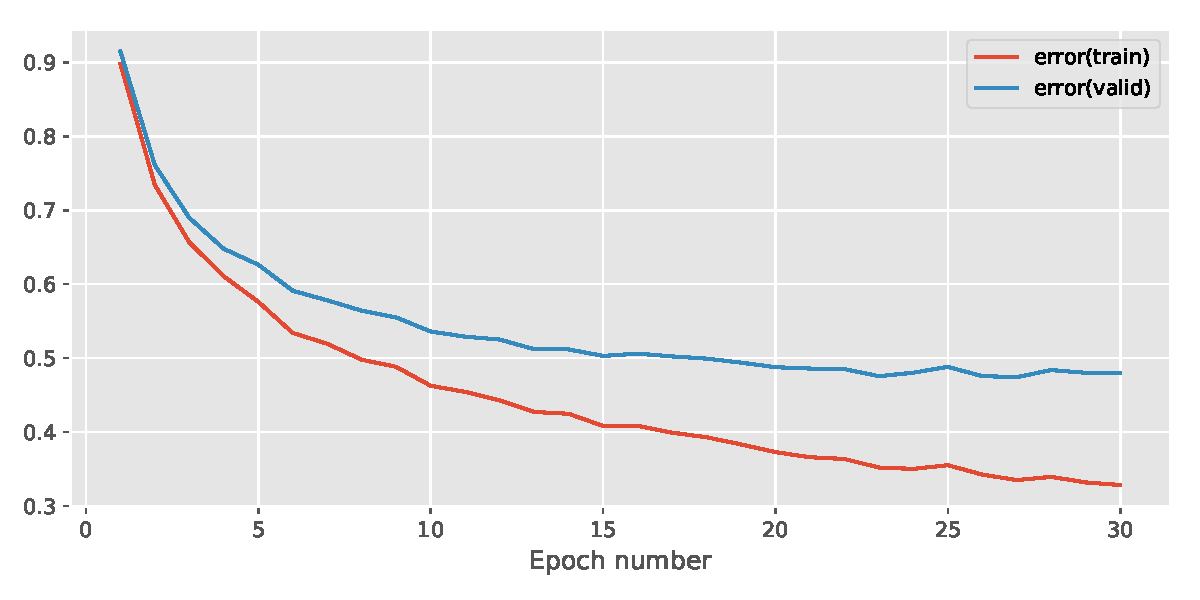
\includegraphics[width=\textwidth]{{../notebooks/figs/adamlearningrulewithweightdecay-cosineannealingwithnorestarts-nonetype-num_epochs100-lr0.0003-n_hidden3_error}.pdf}
		\caption[short]{AdamW noRestart, $lr_{max=0.0003}$}
	\end{subfigure}%
	
	\begin{subfigure}{.45\textwidth}
		\centering
		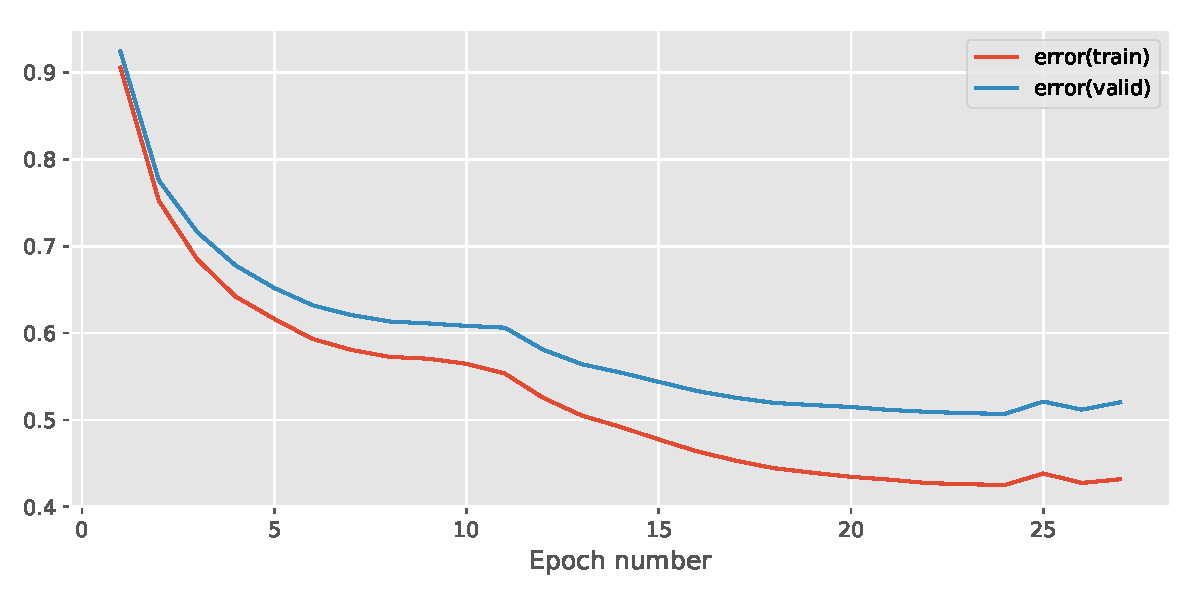
\includegraphics[width=\textwidth]{{../notebooks/figs/adamlearningrulewithweightdecay-cosineannealingwithwarmrestarts-nonetype-num_epochs100-lr0.0003-n_hidden3_error}.pdf}
		\caption[short]{AdamW WarmRestarts, $lr_{max=0.0003}$}
	\end{subfigure}%
	\begin{subfigure}{.45\textwidth}
		\centering
		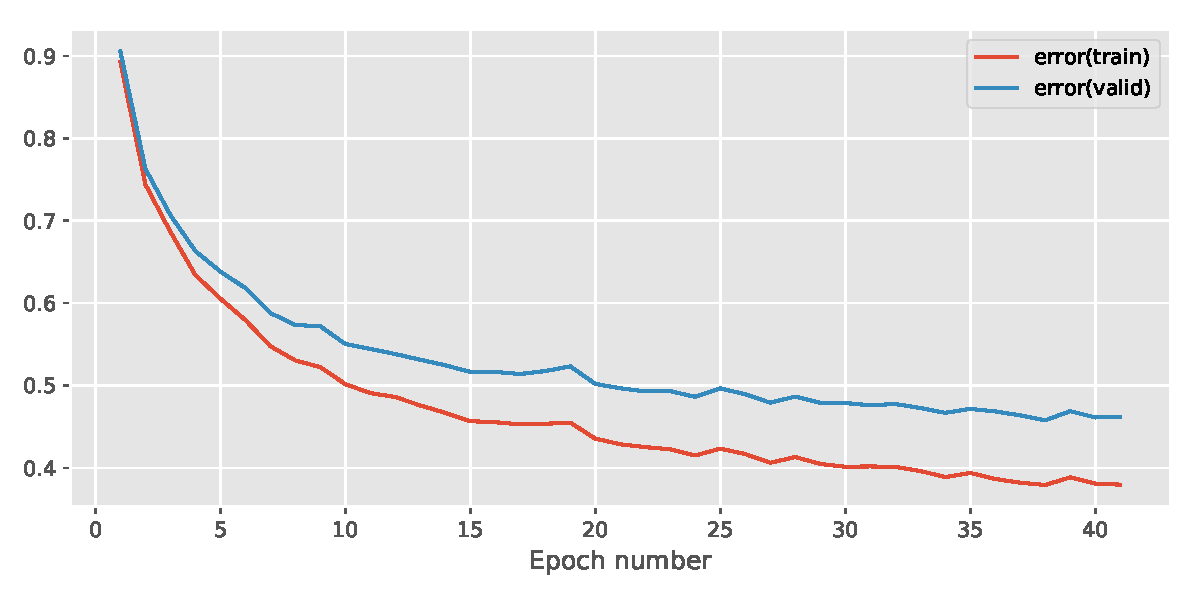
\includegraphics[width=\textwidth]{{../notebooks/figs/adamlearningrule-constantlearningratescheduler-l2penalty-num_epochs100-lr0.0003-n_hidden3_error}.pdf}
		\caption[short]{AdamL2 ConstantLR, $lr_{max=0.0003}$}
	\end{subfigure}%
	
	\begin{subfigure}{.45\textwidth}
		\centering
		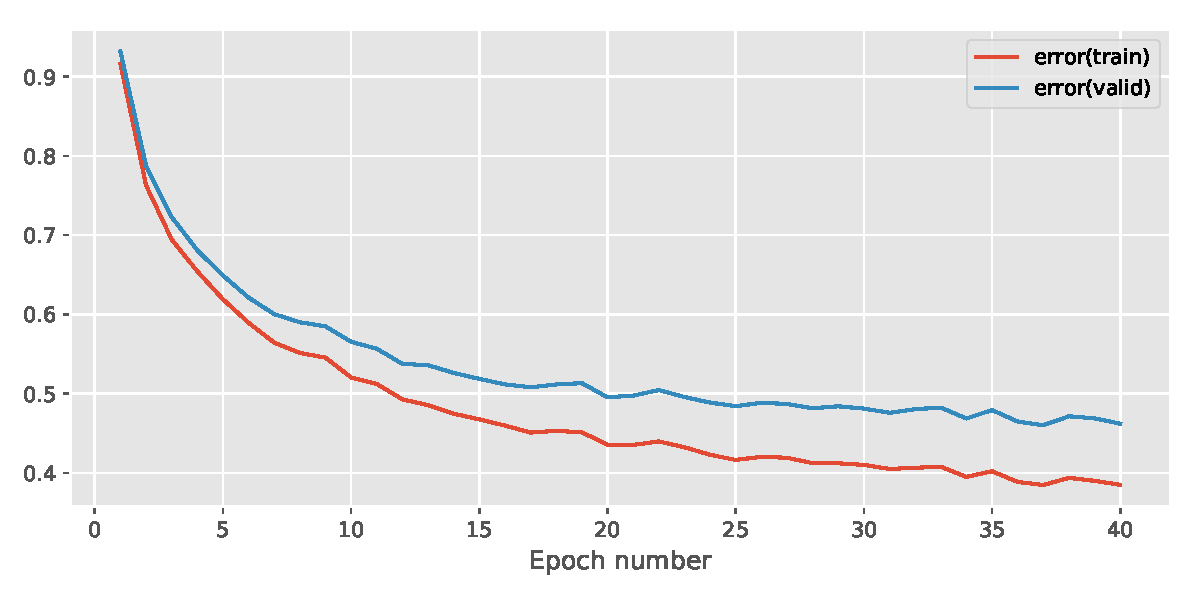
\includegraphics[width=\textwidth]{{../notebooks/figs/adamlearningrule-cosineannealingwithnorestarts-l2penalty-num_epochs100-lr0.0003-n_hidden3_error}.pdf}
		\caption[short]{AdamL2 noRestart, $lr_{max=0.0003}$}
	\end{subfigure}%
	\begin{subfigure}{.45\textwidth}
		\centering
		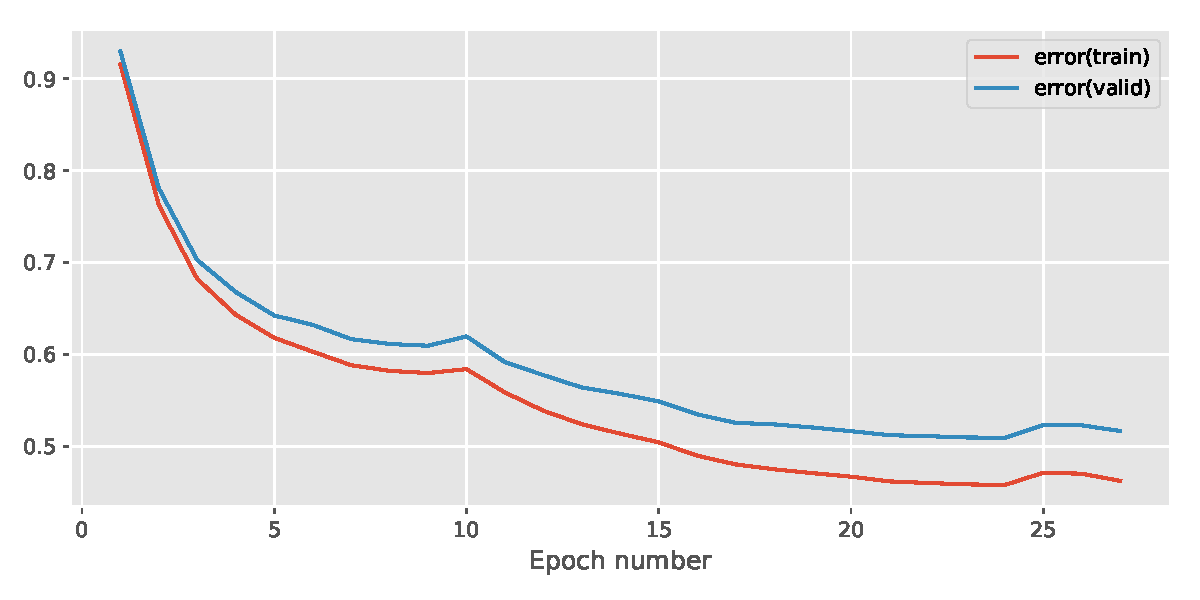
\includegraphics[width=\textwidth]{{../notebooks/figs/adamlearningrule-cosineannealingwithwarmrestarts-l2penalty-num_epochs100-lr0.0003-n_hidden3_error}.pdf}
		\caption[short]{AdamL2 WarmRestarts, $lr_{max=0.0003}$}
	\end{subfigure}%
	\caption[short]{A comparison of no learning rate annealing, annealing with no restart and annealing with restarts. AdamL2 \& AdamW on 3 hidden layer ReLU networks.}
	\label{fig:adamrestart}
\end{figure*}

\end{document} 

